%%%%%%%%%%%%%%%%%%%%%%%%%%%%%%%%%%%%%%%%%%%%%%%%%%%%%%%%%%%%%%%%%%%%%%%%%%%%%%%%
%%
%% Uppsala Beamer theme example by Frédéric Haziza <daz@it.uu.se>
%%
%% Describing beamerthemeUppsala version 2008/05/15
%%
%% If you have more than three sections or more than three subsections in at least
%% one section, you might want to use the [hideallsubsections] or
%% [hideothersubsections] switch.  In this case, only the current (sub-) section is
%% displayed in the sidebar and not the full overview.
%%
%% Options are:
%% ===========
%% * hideallsubsections, hideothersubsections
%% * nonumbers,totalnumber
%% * withnav, mylogo
%% * grey
%% * noprogressbar
%%
%% For the sidebar layout:
%% * subsectionsattop, sectionpathattop
%% 
%% Removed
%% =======
%% * sidebarshades
%%
%% Tip
%% ===
%% latex this file to see the theme in action
%%
%%%%%%%%%%%%%%%%%%%%%%%%%%%%%%%%%%%%%%%%%%%%%%%%%%%%%%%%%%%%%%%%%%%%%%%%%%%%%%%%

\documentclass{beamer}
%\documentclass[handout]{beamer}
%\documentclass[notes]{beamer}
%\documentclass[trans]{beamer}

\usetheme[hideothersubsections]{Uppsala}

\usepackage{hyperref}
\usepackage{pgf}
\usepackage{tikz}
\usepgflibrary{arrows}
\usepgflibrary{shapes}
\usetikzlibrary{%
  arrows,%
  calc,%
  fit,%
  patterns,%
  plotmarks,%
  shapes.geometric,%
  shapes.misc,%
  shapes.symbols,%
  shapes.arrows,%
  shapes.callouts,%
  shapes.multipart,%
  shapes.gates.logic.US,%
  shapes.gates.logic.IEC,%
  er,%
  automata,%
  backgrounds,%
  chains,%
  topaths,%
  trees,%
  petri,%
  mindmap,%
  matrix,%
  calendar,%
  folding,%
  fadings,%
  through,%
  positioning,%
  scopes,%
  decorations.fractals,%
  decorations.shapes,%
  decorations.text,%
  decorations.pathmorphing,%
  decorations.pathreplacing,%
  decorations.footprints,%
  decorations.markings,%
  shadows}

%\usepackage[english]{babel} % or whatever
\usepackage[utf8]{inputenc} % or whatever

\usepackage{mathptmx}
\usepackage{helvet}
%\usepackage{courier}

\usepackage[T1]{fontenc}
% Or whatever. Note that the encoding and the font should match. If T1
% does not look nice, try deleting the line with the fontenc.

\usepackage[makeroom]{cancel}
\usepackage{cwpuzzle}
\usepackage[normalem]{ulem}
\usepackage{multirow,bigdelim}
\usepackage{pgfplots}
\usepackage{pgfplotstable}
\defbeamertemplate{description item}{align left}{\insertdescriptionitem\hfill}
\usepackage{colortbl}
\usepackage{wrapfig}

\usepackage[style=ieee,backend=bibtex]{biblatex}
\addbibresource{astra.bib}
\addbibresource{mybib.bib}
%\bibliography{astra}

%\bibliographystyle{abbrv}
\usepackage{astra}

\newcommand{\Dom}[1]{\text{dom}({#1})}
\newcommand{\Table}{\Constraint{Table}}

% SparseBitSet
\newcommand{\Words}{\texttt{words}}
\newcommand{\Index}{\texttt{index}}
\newcommand{\Mask}{\texttt{mask}}
\newcommand{\Limit}{\texttt{limit}}
\newcommand{\SparseBitSet}{\texttt{SparseBitSet}}
\newcommand{\Offset}{\localvar{offset}}

% CT Propagator
\newcommand{\Scp}{\texttt{vars}}
\newcommand{\CurrTable}{\texttt{validTuples}}
\newcommand{\Sval}{\texttt{S^{val}}}
\newcommand{\Ssup}{\texttt{S^{sup}}}
\newcommand{\LastSizes}{\texttt{lastSize}}
\newcommand{\Supports}{\texttt{supports}}
\newcommand{\Residues}{\texttt{residues}}

% Pseduo code
\newcommand{\ForEach}[1]{\textbf{foreach } {#1} \textbf{ do }}
\newcommand{\ForEachTo}[3]{\textbf{foreach } {#1} \textbf{ from } {#2} 
  \textbf{ to } {#3} \textbf{ do }}
\newcommand{\ForEachDownTo}[3]{\textbf{foreach } {#1} \textbf{ from } {#2} 
  \textbf{ downto } {#3} \textbf{ do }}
\newcommand{\Break}{\textbf{break~}}
\newcommand{\While}[1]{\textbf{while~} {#1} \textbf{~do~}}

\renewcommand{\algorithmicfor}{\textbf{Method}}
\renewcommand{\algorithmicdo}{}
\renewcommand{\algorithmicforall}{\textbf{foreach}}
%\renewcommand{\algorithmicwhile}{\textbf{foreach}}

\newcommand{\Func}[2]{\FOR{#1(#2)}}
\newcommand{\FuncRet}[3]{\FOR{#1(#2) \ : \ \textbf{#3}}}
\newcommand{\Endfunc}{\ENDFOR}
\newcommand{\To}{~\bf{to}~}
\newcommand{\Downto}{~{\bf{downto}}~}
\newcommand{\For}[3]{\FOR{${#1} \leftarrow {#2} \To {#3}$ \textbf{do}}}
\newcommand{\ForDown}[3]{\FOR{${#1} \leftarrow {#2} \Downto {#3}$ \textbf{do}}}
\newcommand{\FOREACH}[1]{\FORALL{{#1} \textbf{do}}}
\newcommand{\ENDFOREACH}{\ENDFOR}

\renewcommand{\algorithmiccomment}[1]{\hfill // #1}
\def\PROCEDURE{\item[\textbf{PROCEDURE}]}
\def\FAILED{\textbf{FAILED}}
\def\NOFIX{\textbf{NOFIX}}
\def\FIX{\textbf{FIX}}
\def\SUBSUMED{\textbf{SUBSUMED}}
\def\FAIL{\textbf{FAIL}}
\def\bool{\mathit{bool}}
\def\StatusMessage{\mathit{StatusMessage}}
\def\FindSupport{\textsc{FindSupport}}
\def\RemoveSupport{\textsc{RemoveSupport}}
\def\Extensional{\textsc{Extensional}}
\def\CompactTable{\textsc{CompactTable}}
\def\UpdateTable{\textsc{UpdateTable}}
\def\FilterDomains{\textsc{FilterDomains}}
\def\FixDomains{\textsc{FixDomains}}
\def\InitialiseCT{\textsc{InitialiseCT}}
\def\IndexOfFixed{\mathit{index\_of\_fixed}}


\newcommand{\ITE}[3]{\text{\bf ~if~} #1 \text{\bf ~then~} #2 \text{\bf ~else~} #3 \text{\bf ~endif}}

\newcommand{\function}[1]{\mathrm{#1}}
\newcommand{\localvar}[1]{\mathit{#1}}

\newlength\myindent
\setlength\myindent{2em}
\newcommand\bindent{%
  \begingroup
  \setlength{\itemindent}{\myindent}
  \addtolength{\algorithmicindent}{\myindent}
}
\newcommand\eindent{\endgroup}

\newcommand{\INDSTATE}[1][1]{\STATE\hspace{#1\algorithmicindent}}
\newcommand{\INDRETURN}[1][1]{\STATE\hspace{#1\algorithmicindent}\textbf{return~}}
\newcommand{\INDIF}[2][1]{\STATE\hspace{#1\algorithmicindent}
  \textbf{if~}{#2}\textbf{~then}}
\newcommand{\INDELSE}[1][1]{\STATE\hspace{#1\algorithmicindent}\textbf{else~}}
\newcommand{\INDELSEIF}[2][1]{\STATE\hspace{#1\algorithmicindent}
  \textbf{else if~}{#2}\textbf{~then}}

\newcommand{\CTpaper}[0]{DBLP:conf/cp/DemeulenaereHLP16}

\newcommand{\stressed}[1]{\emph{{\color{red!50}{#1}}}}

%% -----------------------------------------------------------
%% MISC. INFORMATION
%% -----------------------------------------------------------

\title{Implementation and Evaluation of a Compact-Table Propagator in Gecode}
%\subtitle{Bachelor's thesis}

\author[Linnea Ingmar | \emph{linnea.ingmar.3244@student.uu.se}] % appears in the footline
{Linnea Ingmar \\ <\texttt{linnea.ingmar.3244@student.uu.se}>}


\institute[Dept. of Information Technology] % appears in the footline
{
  The ASTRA Group\\ on Combinatorial Optimisation \\
  Uppsala University
}


\date[\today] % appears in the bottom of the sidebar
{\today}

%% \logo{...}

%% This is only inserted into the PDF information catalog. Can be left out.
\subject{Unofficial Beamer Theme for Uppsala University}

%% -----------------------------------------------------------
%% Extra ``local'' settings
%% -----------------------------------------------------------

% Comment out this, if you do not want the table of contents to pop up at
% the beginning of each (sub)section:
\AtBeginSection[]
{
  \begin{frame}<beamer> % with <beamer> => doesn't appear in handout mode
    \frametitle{Outline} %% Put the title you want, or none!
    %\tableofcontents[currentsection,currentsubsection]
    \tableofcontents[currentsection]
  \end{frame}
}

%% Unfolds piecewise element with shading.
%% Text appears, shaded, and the audience knows that somehting is coming
%% Note: if you set the number too high, the audience will try to read the 
%% text that now shows up more, and will be disturbed.
%% ``dynamic'' makes elements show gradually more and more.
\setbeamercovered{transparent=5}
%% \setbeamercovered{dynamic=5}

%% -----------------------------------------------------------

\begin{document}

\begin{frame}[plain] %% Gets the frame to fill up the page, no menu/sidebar/footline
  \titlepage
  
  \begin{figure}
    \begin{flushright}
        \begin{tabular}[t,right]{lr}
          Supervisor: & Mats Carlsson \\
          Reviewer:   & Pierre Flener
        \end{tabular}
      \end{flushright}
  \end{figure}

\end{frame}

\begin{frame}
    \frametitle{Outline}
    \tableofcontents[currentsection]
\end{frame}

\section{Background}

%\subsection{Constraint Programming}

\begin{frame}
  \frametitle{Kakuro puzzle}
  \begin{minipage}{0.45\textwidth}
    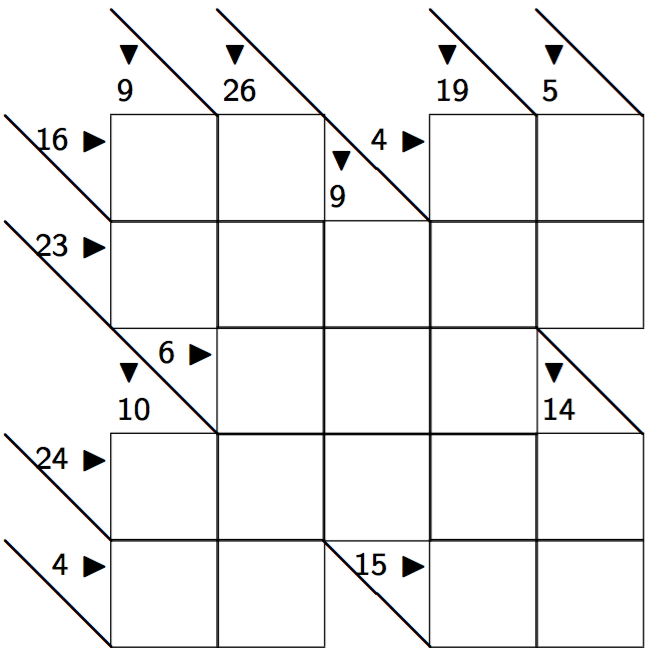
\includegraphics[scale=0.15]{kakuro.png}
  \end{minipage}
  \begin{minipage}{0.45\textwidth}
    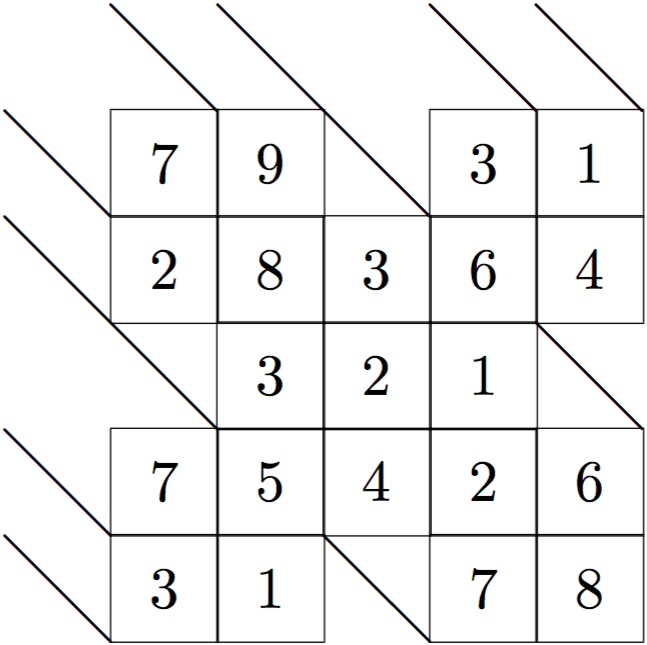
\includegraphics[scale=0.15]{kakuro-sol.png}
  \end{minipage}

  \bigskip

  Assign the cells digits from~$1$ to~$9$ such that for each row and column:
  \begin{itemize}
    \item digits are distinct, and
    \item the sum of the digits is equal to the \emph{clue}
    \end{itemize}

\end{frame}

\begin{frame}
  \frametitle{Kakuro puzzle as a constraint problem (1)}
  \begin{minipage}{0.6\textwidth}
    \begin{description}
      \item[Variables] One per cell.
      \item[Domains] $\Set{1...9}$ for all variables.
      \item[Constraints] For each row and column: \stressed{distinct} digits,
        and the \stressed{sum} of the digits is equal to the clue.
    \end{description} 
  \end{minipage}
  \begin{minipage}{0.35\textwidth}
    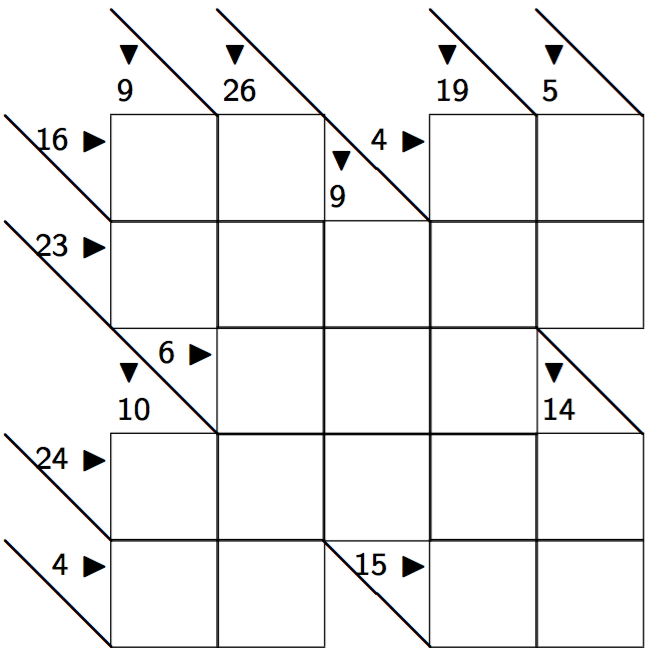
\includegraphics[scale=0.15]{kakuro.png}
  \end{minipage}
\end{frame}

\begin{frame}
  \frametitle{Kakuro puzzle as a constraint problem (2)}
  \begin{minipage}{0.6\textwidth}
    \begin{description}
      \item[Variables] One per cell.
      \item[Domains] $\Set{1...9}$ for all variables.
      \item[Constraints] For each row and column: state the \stressed{possible
        combinations of values} that the variables can take.
    \end{description} 
  \end{minipage}
  \begin{minipage}{0.35\textwidth}
    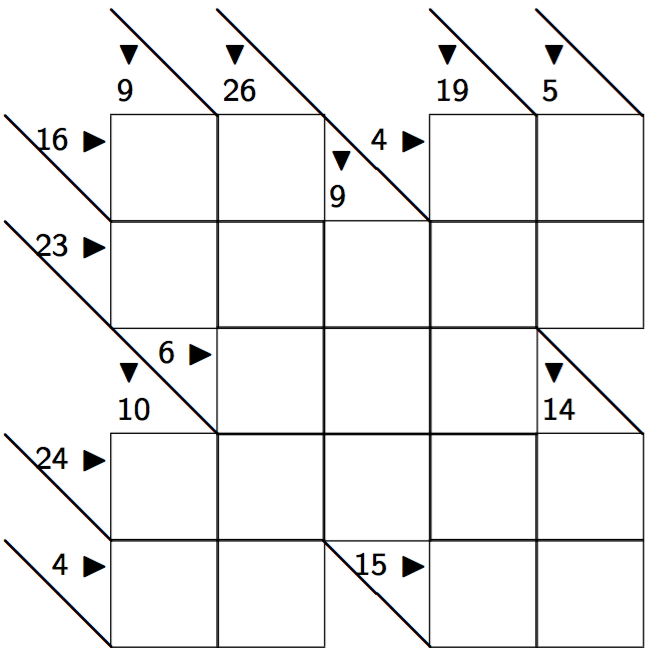
\includegraphics[scale=0.15]{kakuro.png}
  \end{minipage}

  \bigskip
  \bigskip
  Row/column of size~$2$ and clue~$16$:~$\Tuple{7,9}$ and~$\Tuple{9,7}$
  are the only combinations.
\end{frame}

\begin{frame}
  \frametitle{\Table~constraints}
  \begin{definition}[\Table~constraint]
    A \Table~constraint lists the possible combinations of values
    that the variables can take as a sequence of~$n$-tuples.
  \end{definition}

  \bigskip
  \bigskip

  \begin{tabular}{lccr}
    %\Table($\Set{x_0,x_1}$, $[\Tuple{7,9},\Tuple{9,7}]$)\\
    \bigskip
    \begin{tabular}{cc}
      $x_0$ & $x_1$ \\
      \hline
      $7$   & $9$ \\
      $9$   & $7$ \\
    \end{tabular}
            &
            &
            &
              \phantom{foo}
              \includegraphics[scale=0.2]{kakuro-hint.png}
    
  \end{tabular}
\end{frame}



% - CSP
% \begin{frame}
%   \frametitle{Constraint problems (definition)}
%   \begin{definition}[Constraint problem]
%     A \textbf{constraint satisfaction problem (CSP)} is a 
%     triple\\
%     \begin{center}
%       $\left<V,D,C\right>$\\      
%     \end{center}
%     where: \\
%     \begin{itemize}
%       \item $V = v_1, \ldots, v_n$ is a finite sequence of variables,
%       \item $D = D_1, \ldots, D_n$ is a finite sequence of domains, that are
%         possible values for the respective variable,
%       \item $C = \Set{c_1, \ldots, c_m}$ is a finite set of constraints, 
%         each on a subset of~$V$. 
%         Express relations among the variables that have to be true.
%     \end{itemize}
%   \end{definition}
% \end{frame}

\begin{frame}
  \frametitle{Solving Constraint Problems}
  \begin{minipage}{0.6\textwidth}
    \begin{description}
    \item[Solution]
      A complete
      variable-value assignment satisfying the constraints.\\
      \smallskip
      (Sometimes: maximises/minimises given function.)
    \end{description}
  \end{minipage}
  \begin{minipage}{0.35\textwidth}
    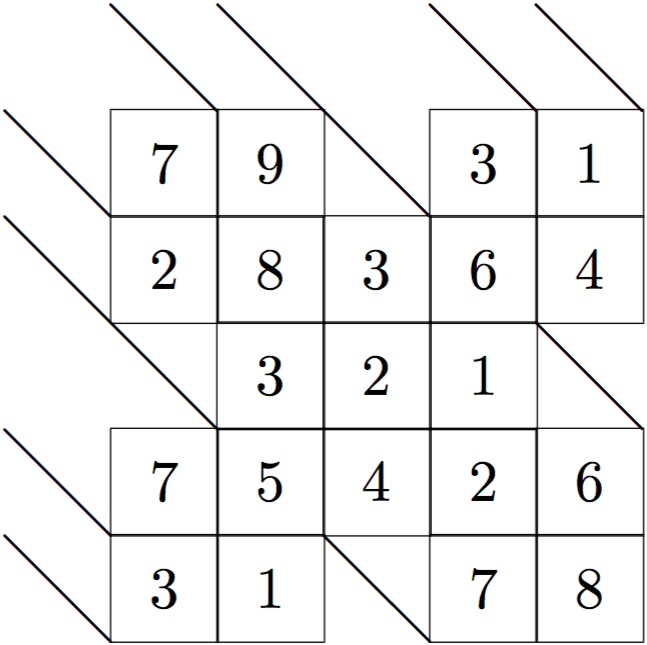
\includegraphics[scale=0.15]{kakuro-sol.png} \\
  \end{minipage}
  
  \begin{minipage}{0.6\textwidth}
    \begin{itemize}
    \item Solutions are found by \textbf{search}
      \begin{itemize}
      \item \alt<2>{\textbf{Propagation}}{Propagation}
      \item \alt<2>{\color{gray}Branching}{Branching}
      \end{itemize}
    \end{itemize}
  \end{minipage}
  \begin{minipage}{0.15\textwidth}
    \includegraphics[scale=0.3]{searchtree.png}
  \end{minipage}
  % \begin{minipage}{0.15\textwidth}
  %   \tiny
  %   \begin{tabular}[t]{c}
  %     Propagation \\
  %     Branching \\
  %     Propagation \\
  %     Branching \\
  %   \end{tabular}
  % \end{minipage}
  
\end{frame}


% - Store

\begin{frame}
  \frametitle{Constraint Propagation}
  Important concepts:
  \begin{itemize}
    \item Constraint store
    \item Propagator
    %\item Constraint propagation
  \end{itemize}
\end{frame}

\begin{frame}
  \frametitle{Constraint Stores}
  \begin{definition}[Constraint store]
    A \textbf{constraint store}~$s$ is a function mapping variables
    to domains:
    \begin{center}
      $s: variables \mapsto domains$
    \end{center}
  \end{definition}

  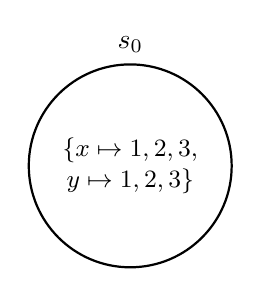
\begin{tikzpicture}[->,>=stealth',auto,node distance=3cm,
    thick,main node/.style={circle,draw,font=\sffamily\Large\bfseries}]
    \node[label={$s_0$},draw,circle](1){
      \small
      \begin{tabular}{c}
        $\{x \mapsto \Set{1,2,3},$\\ 
        $y\mapsto\Set{1,2,3}\}$
      \end{tabular}
    };
    
  \end{tikzpicture}

\end{frame}

\begin{frame}
  \frametitle{Propagators}
  \begin{definition}[Propagator]
    A \textbf{propagator}~$p$ is a function mapping stores to stores:
    \begin{center}
      $p: store \mapsto store$ 
    \end{center}
  \end{definition}

  \begin{itemize}
  \item   Implement constraints
  % \item   Prune values from the domains that are in conflict 
  %   with the constraint
  \end{itemize}

  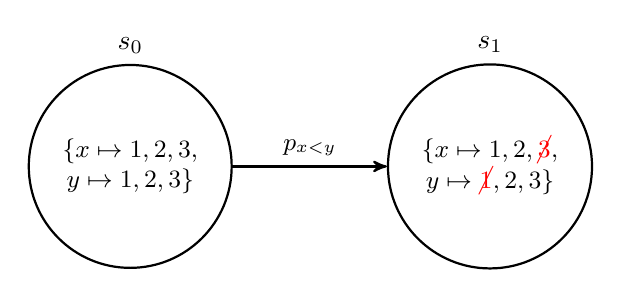
\begin{tikzpicture}[->,>=stealth',auto,node distance=3cm,
  thick,main node/.style={circle,draw,font=\sffamily\Large\bfseries}]
    \node[label=$s_0$,draw,circle](1){
      \small
      \begin{tabular}{c}
        $\{x \mapsto \Set{1,2,3},$\\ 
        $y\mapsto\Set{1,2,3}\}$
      \end{tabular}
    };
    \node[label=$s_1$,draw,circle,right of=1,node distance=13em](2){
      \small
      \begin{tabular}{c}
        $\{x \mapsto \Set{1,2,{\color{red}\cancel{3}}},$\\ 
        $y\mapsto\Set{{\color{red}\cancel{1}},2,3}\}$
      \end{tabular}
    };
    \path[every node/.style={font=\sffamily\small}] 
    (1) edge node [bend right] {$p_{x<y}$} (2);
    
  \end{tikzpicture}

\end{frame}

\begin{frame}
  \frametitle{Constraint Propagation}
  %Prune values from the variables that  
  \begin{minipage}{0.5\textwidth}
    \only<1>{$x_0 \in \Set{1,2,3,4,5,6,7,8,9}$}
    \only<2>{$x_0 \in \Set{\cancel{\color{blue}1},\cancel{\color{blue}2},\cancel{\color{blue}3},\cancel{\color{blue}4},\cancel{\color{blue}5},\cancel{\color{blue}6},7,\cancel{\color{blue}8},9}$}
    \only<3->{$x_0 \in \Set{\cancel{\color{blue}1},\cancel{\color{blue}2},\cancel{\color{blue}3},\cancel{\color{blue}4},\cancel{\color{blue}5},\cancel{\color{blue}6},\textbf{7},\cancel{\color{blue}8},\cancel{\color{purple}9}}$} \\
    \only<1>{$x_1 \in \Set{1,2,3,4,5,6,7,8,9}$}
    \only<2-3>{$x_1 \in \Set{\cancel{\color{blue}1},\cancel{\color{blue}2},\cancel{\color{blue}3},\cancel{\color{blue}4},\cancel{\color{blue}5},\cancel{\color{blue}6},7,\cancel{\color{blue}8},9}$}
    \only<4->{$x_1 \in \Set{\cancel{\color{blue}1},\cancel{\color{blue}2},\cancel{\color{blue}3},\cancel{\color{blue}4},\cancel{\color{blue}5},\cancel{\color{blue}6},\cancel{\color{blue}7},\cancel{\color{blue}8},\textbf{9}}$}\\
    $\ldots$ \\
    \only<1-2>{$x_4 \in \Set{1,2,3,4,5,6,7,8,9}$}
    \only<3->{$x_4 \in \Set{\cancel{\color{purple}1},\textbf{2},\cancel{\color{purple}3},\cancel{\color{purple}4},\cancel{\color{purple}5},\cancel{\color{purple}6},\cancel{\color{purple}7},\cancel{\color{purple}8},\cancel{\color{purple}9}}$}\\
    $\ldots$
    %$\Table(\Set{x_0,x_1},\Set{\Tuple{7,9},\Tuple{9,7}})$
    
    \begin{tabular}{ccc}
      
      \begin{tabular}{!{\color{blue}\vrule}cc!{\color{blue}\vrule}}
        \arrayrulecolor{blue}\hline
        $x_0$ & $x_1$ \\
        \hline
        $7$   & $9$ \\
        \alt<4>{\sout{$9$}   & \sout{$7$}} 
                               {$9$   & $7$} \\
        \arrayrulecolor{blue}\hline
        
      \end{tabular} & 
                         \only<1>{
                          \begin{tabular}{!{\color{purple}\vrule}cc!{\color{purple}\vrule}}
                            \arrayrulecolor{purple}\hline
                            $x_0$ & $x_4$ \\
                            \hline
                            $1$   & $8$ \\
                            $2$   & $7$ \\
                            $3$   & $6$ \\
                            $4$   & $5$ \\
                            $5$   & $4$ \\
                            $6$   & $3$ \\
                            $7$   & $2$ \\
                            $8$   & $1$ \\
                            \arrayrulecolor{purple}\hline
                          \end{tabular} & $\ldots$}
                          \only<2->{
                          \begin{tabular}{!{\color{purple}\vrule}cc!{\color{purple}\vrule}}
                            \arrayrulecolor{purple}\hline
                            $x_0$ & $x_4$ \\
                            \hline
                            \sout{$1$}   & \sout{$8$} \\
                            \sout{$2$}   & \sout{$7$} \\
                            \sout{$3$}   & \sout{$6$} \\
                            \sout{$4$}   & \sout{$5$} \\
                            \sout{$5$}   & \sout{$4$} \\
                            \sout{$6$}   & \sout{$3$} \\
                            $7$   & $2$ \\
                            \sout{$8$}  &  \sout{$1$}\\
                            \arrayrulecolor{purple}\hline
                          \end{tabular} & $\ldots$}

    \end{tabular}

  \end{minipage}
  \begin{minipage}{0.45\textwidth}
    \alt<4>
    {\includegraphics[scale=0.2]{kakuro-vars-color-ass.png}}
    {\includegraphics[scale=0.2]{kakuro-vars-color.png}}

  \end{minipage}
\end{frame}

%\subsection{Gecode}

\begin{frame}

 
  \frametitle{Gecode}
  \textbf{Gecode} (Generic Constraint Development Environment)

  \begin{itemize}
    \item A constraint solver (a software that solves constraint problems).
    \item Written in C++, modular, extensible, and has state-of-the-art performance.
    \item Supports the programming of new propagators.
    \item Uses copying during branching, not trailing
    \item   Two existing propagators for the~\Table~constraint
  \end{itemize}

  % , and one for the 
  % related constraint~\Constraint{Regular}.
  
    \begin{figure}[t]
    \begin{center}
      \includegraphics[scale=0.25]{gecode.png}
    \end{center}
  \end{figure}


\end{frame}

%\subsection{The Compact-Table algorithm}

\begin{frame}
  \frametitle{Compact Table}
  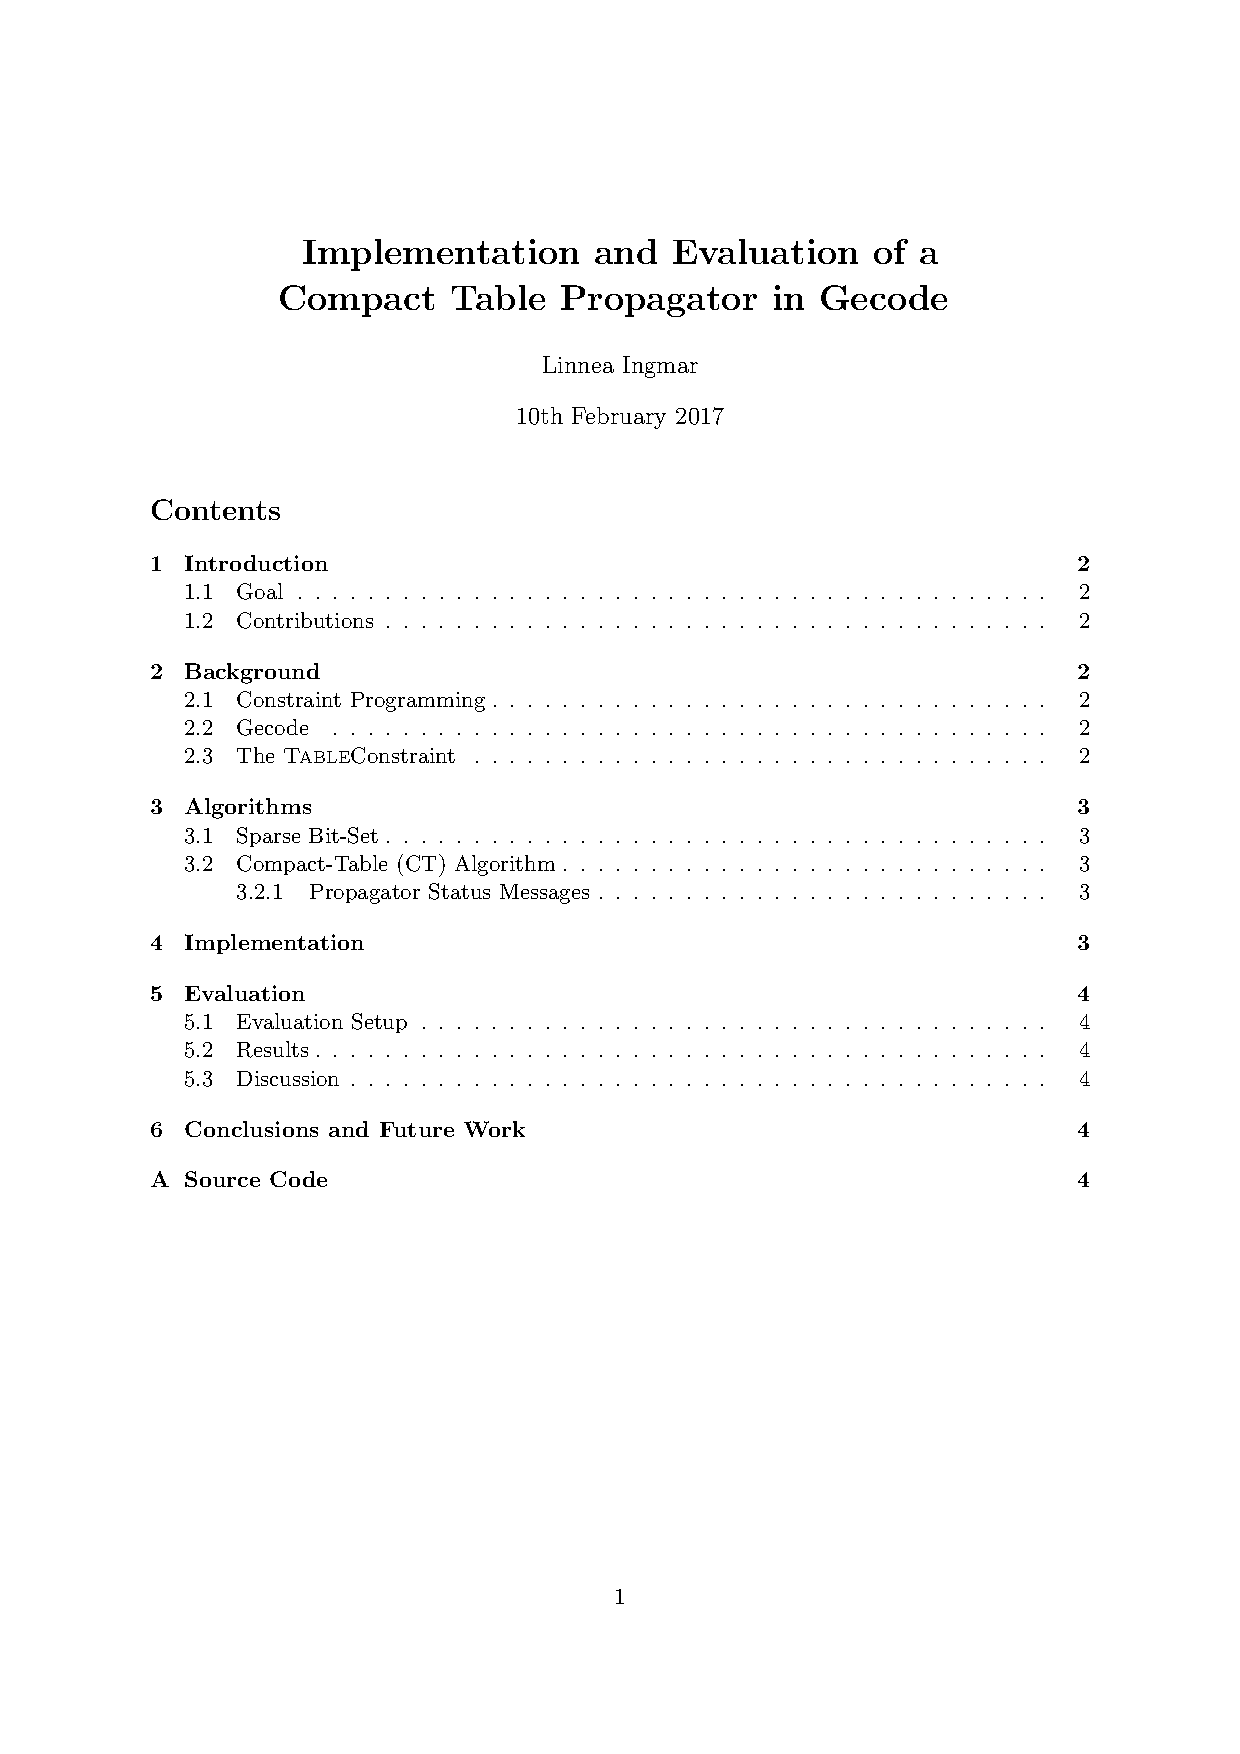
\includegraphics[scale=0.45]{compact-table.png}
\end{frame}

\begin{frame}
  \frametitle{Compact-Table}
  % Efficient
  \begin{itemize}
  \item   A new propagation algorithm for the~\Table~constraint
  \item   First implemented in OR-tools (uses trailing during branching)
  \item   Published in a 2016 paper~\cite{\CTpaper} -- the starting
    point of this project
  \item   Promising results - outperforms previously known algorithms in the
    benchmarks in \cite{\CTpaper}
  \item   No attempt to implement it in Gecode (until now)
  \end{itemize}

\end{frame}

\section{The Compact-Table Algorithm}

% \begin{frame}
%   \frametitle{Fields}
%   \begin{description}
%     \item[\CurrTable] \emph{Sparse bit-set:} Stores indices of valid tuples
%     \item[\Supports]  \emph{Array of bit-sets:} \Supports[$x,a$] stores which tuples
%       are supports for the variable-value pair~$\Tuple{x,a}$
%     \item[\Residues]  \emph{Array of ints:} $\Residues[x,a]$ is the index in \CurrTable~where
%       a support for~$\Tuple{x,a}$ was found the last time it was sought for
%   \end{description}
%   \bigskip
%   % Where:
%   % \emph{Valid tuple~:} All values in~$\tau$ are in the domains of the variables
%   % \emph{Support:} $\tau$ is a support for  

% \end{frame}

% \begin{frame}
%   \frametitle{The Compact-Table Algorithm}
%   \begin{itemize}
%   \item \textbf{Initialisation}
%   \item \color{gray}Variable modifications
%   \item Filtering
%    \item {\color{gray}Putting it all together}
%   \end{itemize}
% \end{frame}

\begin{frame}
%  \frametitle{The Compact-Table Algorithm}
  \frametitle{Initialisation}
  \small
  \only<1-5>{
    $\Dom{x_0} = \Dom{x_1} = \Dom{x_2} = \Set{1,2,3,4}$
  }
  \only<6->{
    $\Dom{x_0} = \Set{1,2,{\color{red}\cancel{3}},4}$\\
    $\Dom{x_1} = \Dom{x_2} = \Set{1,2,3,4}$
  }

  \bigskip

  \begin{tabular}{l}

    \only<4->{
    %\CurrTable: bit-set with valid tuples\\
    %\phantom{foo}\\
    \small
    \begin{tabular}{cc}
      %\phantom{\texttt{words}}
      \phantom{$\Tuple{x_0,2}$}
      &
        \begin{tabular}{|cccccccc|c}
          \cline{1-8}
          {\textbf{1}} & {\textbf{1}} & {\textbf{1}} & {\textbf{1}} & {\textbf{1}}& {\textbf{1}}& {\textbf{1}} & {\textbf{1}} & \rdelim\}{1}{3mm}[\CurrTable] \\
          \cline{1-8}
        \end{tabular}
    \end{tabular}

    \bigskip
    }
    \\
    \only<5->{
    %\Supports: \\
    %\phantom{foo}\\
    \begin{tabular}{ccc}
      $\Tuple{x_0,1}$
      & 
        \begin{tabular}{|cccccccc|}
          \hline
          0 & \textbf{1} & 0 & 0 & \textbf{1} & 0 & 0 & 0 \\
        \end{tabular}
      &
        \rdelim\}{5}{3mm}[\texttt{supports}]
      \\
      $\Tuple{x_0,2}$
      & 
        \begin{tabular}{|cccccccc|}
          \textbf{1} & 0 & \textbf{1} & 0 & 0 & \textbf{1} & \textbf{1} & 0 \\
        \end{tabular}
      \\
      $\Tuple{x_0,3}$
      & 
        \begin{tabular}{|cccccccc|}
          \alt<6->{{\color{red}0} & \color{red}0 & \color{red}0 & \color{red}0 & \color{red}0 & \color{red}0 & \color{red}0 & {\color{red}0}} 
              {0 & 0 & 0 & 0 & 0 & 0 & 0 & 0} \\
          
        \end{tabular}
      \\
      $\ldots$
      \\
      $\Tuple{x_2,4}$
      & 
        \begin{tabular}{|cccccccc|}
          \textbf{1} & 0 & 0 & 0 & 0 & 0 & 0 & 0 \\
          \hline
        \end{tabular}
      \\
    \end{tabular}
        
    \bigskip
    } 
    \\
    \only<1>{
    \small
        \begin{tabular}{|c|cccccccccccccccc|}
          \hline
          $x_0$ & 1 & 2 & 1 & 2 & 6 & 7 & 4 & 1 & 7 & 8 & 2 & 0 & 2 & 5 & 4 \\
          $x_1$ & 5 & 1& 3 & 4 & 5 & 7 & 2 & 1 & 8 & 9 & 2 & 0 & 3 & 8 & 3 \\
          $x_2$ & 8 & 4& 2 & 2 & 9 & 8 & 1 & 1 & 9 & 6 & 3 & 0 & 1 & 5 & 1 \\
          \hline
        \end{tabular}}
    \only<2>{
    \small
    \begin{tabular}{|c|ccccccccccccccc|}
      \hline
      $x_0$ & 1 & \textbf{2} & \textbf{1} & \textbf{2} & 6 & 7 & \textbf{4} & \textbf{1} & 7 & 8 & \textbf{2} & 0 & \textbf{2} & 5 & \textbf{4} \\
      $x_1$ & 5 & \textbf{1}& \textbf{3} & \textbf{4} & 5 & 7 & \textbf{2} & \textbf{1} & 8 & 9 & \textbf{2} & 0 & \textbf{3} & 8 & \textbf{3} \\
      $x_2$ & 8 & \textbf{4}& \textbf{2} & \textbf{2} & 9 & 8 & \textbf{1} & \textbf{1} & 9 & 6 & \textbf{3} & 0 & \textbf{1} & 5 & \textbf{1} \\
      \hline
    \end{tabular}
    }
    
    \small
    \begin{tabular}{cc}
      &
        \only<3->{
        \begin{tabular}{|c|cccccccc|}
          \hline
          $x_0$ & \textbf{2}& \textbf{1} & \textbf{2} & \textbf{4} & \textbf{1} & \textbf{2} & \textbf{2} & \textbf{4} \\
          $x_1$ & \textbf{1}& \textbf{3} & \textbf{4} & \textbf{2} & \textbf{1} & \textbf{2} & \textbf{3} & \textbf{3} \\
          $x_2$ & \textbf{4}& \textbf{2} & \textbf{2} & \textbf{1} & \textbf{1} & \textbf{3} & \textbf{1} & \textbf{1} \\
          \hline
          \multicolumn{1}{c}{} &
          \multicolumn{1}{c}{\tiny 0} &
          \multicolumn{1}{c}{\tiny 1}&
          \multicolumn{1}{c}{\tiny 2}&
          \multicolumn{1}{c}{\tiny 3}&
          \multicolumn{1}{c}{\tiny 4}&
          \multicolumn{1}{c}{\tiny 5}&
          \multicolumn{1}{c}{\tiny 6}&
          \multicolumn{1}{c}{\tiny 7}
        \end{tabular}
      }

    \end{tabular}

  \end{tabular}

\end{frame}


% \begin{frame}
%   \frametitle{The Compact-Table Algorithm}
%   \begin{itemize}
%   \item {\color{gray}Initialisation}
%   \item \textbf{Variable modifications}
%   \item {\color{gray}Filtering}
%   \item {\color{gray}Putting it all together}
%   \end{itemize}
% \end{frame}
\begin{frame}
  \frametitle{Variable Modifications}
  When a variable~$x$ is modified, there are two ways to update~\CurrTable:
  \smallskip
  \begin{description}
    \item[$\Cardinality{\Delta_x} < \Cardinality{\Dom{x}}$] Reset-based update
    \item[$\Cardinality{\Delta_x} \geq \Cardinality{\Dom{x}}$] Incremental update
  \end{description}

  \bigskip
  \bigskip

  \begin{tabular}{|c|}
    \hline
    $\Delta_x$: set of removed values \\
    \hline
  \end{tabular}

\end{frame}

\begin{frame}
  %\frametitle{The Compact-Table Algorithm}
  \frametitle{Variable Modifications}
  \framesubtitle{Reset-based update}

  \only<2->{
    \begin{tabular}{c}
      \small
      \begin{tabular}{ccc}
        \texttt{words} 
        & 
          \begin{tabular}{|cccccccc|}
            \hline
            \alt<7->{{\color{red}0} & {\textbf{1}} & {\textbf{1}} & {\color{red}0} & {\color{red}0}& {\color{red}0}& {\textbf{1}} & {\textbf{1}}}
            {{\textbf{1}} & {\textbf{1}} & {\textbf{1}} & {\textbf{1}} & {\textbf{1}}& {\textbf{1}}& {\textbf{1}} & {\textbf{1}}} \\
            \hline
          \end{tabular}
        &
          \rdelim\}{2}{1mm}[\tiny \CurrTable]
        \\
        \texttt{mask} 
        &
          \begin{tabular}{|cccccccc|}
            \hline
            \alt<5->{{0} & {\textbf{1}} & {\textbf{1}} & {0} & {0}& {0}& {\textbf{1}} & {\textbf{1}}}
            {{0} & {0} & {0} & {0} & {0}& {0}& {0} & {0}} \\
            \hline
          \end{tabular} 
        \\
        \only<3->{
        \phantom{foo} \\
        $\Supports[x_1,3]$ 
        & 
          \begin{tabular}{|cccccccc|}
            \hline
            0 & \textbf{1} & 0 & 0 & 0 & 0 & \textbf{1} & \textbf{1} \\
            \hline
          \end{tabular}
        \\
        $\Supports[x_1,4]$
        & 
          \begin{tabular}{|cccccccc|}
            \hline
            0 & 0 & \textbf{1} & 0 & 0 & 0 & 0 & 0 \\
            \hline
          \end{tabular}
        \\
        }
        \only<8->{
        \phantom{foo} \\
        $x_0$
        &
          \small
          \begin{tabular}{|cccccccc|}
            \hline
            {\color{red}2}& \textbf{1} & \textbf{2} & {\color{red}4} & {\color{red}1} & {\color{red}2} & \textbf{2} & \textbf{4} \\
          \end{tabular}
        \\
        $x_1$
        &
          \small
          \begin{tabular}{|cccccccc|}
            {\color{red}1}& \textbf{3} & \textbf{4} & {\color{red}2} & {\color{red}1} & {\color{red}2} & \textbf{3} & \textbf{3} \\
          \end{tabular}
        \\
        $x_2$
        &
        \small
          \begin{tabular}{|cccccccc|}
            {\color{red}4}& \textbf{2} & \textbf{2} & {\color{red}1} & {\color{red}1} & {\color{red}3} & \textbf{1} & \textbf{1} \\
            \hline
          \end{tabular}
        \\
        }
      \end{tabular}
      \\
      \only<4>{
      \phantom{foo}\\
      \texttt{mask} = \Supports[$x_1,3$] | \Supports[$x_1,4$]\\
      }
      \only<6>{
        \phantom{foo}\\
      \small
      \texttt{words} = \texttt{words} \& \texttt{mask} \\
      }
    \end{tabular}
    \\
  }
  
  \bigskip

  $\Dom{x_0} = \Set{1,2,4}$\\
  $\Dom{x_1} = \Set{\cancel{1},\cancel{2},3,4}$\\
  $\Dom{x_2} = \Set{1,2,3,4}$

\end{frame}

\begin{frame}
  %\frametitle{The Compact-Table Algorithm}
  \frametitle{Variable Modifications}
  \framesubtitle{Incremental update}

  \only<2->{
    \begin{tabular}{c}
      \small
      \begin{tabular}{ccc}
        \texttt{words} 
        & 
          \begin{tabular}{|cccccccc|}
            \hline
            \alt<7->{{\color{red}0} & {\textbf{1}} & {\textbf{1}} & {\color{red}0} & {\color{red}0}& {\color{red}0}& {\textbf{1}} & {\textbf{1}}}
            {{\textbf{1}} & {\textbf{1}} & {\textbf{1}} & {\textbf{1}} & {\textbf{1}}& {\textbf{1}}& {\textbf{1}} & {\textbf{1}}} \\
            \hline
          \end{tabular}
        &
          \rdelim\}{2}{1mm}[\tiny \CurrTable]
        \\
        \texttt{mask} 
        &
          \begin{tabular}{|cccccccc|}
            \hline
            \alt<5->{\textbf{1} & 0 & 0 & \textbf{1} & \textbf{1} & \textbf{1} & 0 & 0}
            {{0} & {0} & {0} & {0} & {0}& {0}& {0} & {0}} \\
            \hline
          \end{tabular} 
        \\
        \only<3->{
        \phantom{foo} \\
        $\Supports[x_1,1]$ 
        & 
          \begin{tabular}{|cccccccc|}
            \hline
            \textbf{1} & 0 & 0 & 0 & \textbf{1} & 0 & {0} & {0} \\
            \hline
          \end{tabular}
        \\
        $\Supports[x_1,2]$
        & 
          \begin{tabular}{|cccccccc|}
            \hline
            0 & 0 & {0} & \textbf{1} & 0 & \textbf{1} & 0 & 0 \\
            \hline
          \end{tabular}
        \\
        }
        \only<8->{
        \phantom{foo} \\
        $x_0$
        &
          \small
          \begin{tabular}{|cccccccc|}
            \hline
            {\color{red}2}& \textbf{1} & \textbf{2} & {\color{red}4} & {\color{red}1} & {\color{red}2} & \textbf{2} & \textbf{4} \\
          \end{tabular}
        \\
        $x_1$
        &
          \small
          \begin{tabular}{|cccccccc|}
            {\color{red}1}& \textbf{3} & \textbf{4} & {\color{red}2} & {\color{red}1} & {\color{red}2} & \textbf{3} & \textbf{3} \\
          \end{tabular}
        \\
        $x_2$
        &
        \small
          \begin{tabular}{|cccccccc|}
            {\color{red}4}& \textbf{2} & \textbf{2} & {\color{red}1} & {\color{red}1} & {\color{red}3} & \textbf{1} & \textbf{1} \\
            \hline
          \end{tabular}
        \\
        }
      \end{tabular}
      \\
      \only<4>{
      \phantom{foo}\\
      \texttt{mask} = \Supports[$x_1,1$] | \Supports[$x_1,2$]\\
      }
      \only<6>{
        \phantom{foo}\\
      \small
      \texttt{words} = \texttt{words} \& !\texttt{mask} \\
      }
    \end{tabular}
    \\
  }
  
  \bigskip

  $\Dom{x_0} = \Set{1,2,4}$\\
  $\Dom{x_1} = \Set{\cancel{1},\cancel{2},3,4}$\\
  $\Dom{x_2} = \Set{1,2,3,4}$

\end{frame}


\begin{frame}
  %\frametitle{Compact-Table Algorithm}
  \frametitle{Filtering}
    
  \begin{itemize}
    \item Intersect every support entry with~$\CurrTable$
    \item Remove value if intersection is empty
  \end{itemize}
  
  \bigskip

  \begin{tabular}{c}
      \CurrTable:\\
      \small
      \begin{tabular}{cc}
        \texttt{words} 
        & 
          \begin{tabular}{|cccccccc|}
            \hline
            {0} & {\textbf{1}} & {\textbf{1}} & {0} & {0} & {0} & {\textbf{1}} & {\textbf{1}} \\
            \hline
          \end{tabular}
      \end{tabular} \\
    \\
    \& \\
    \phantom{foo}
    \\
    \small
    \begin{tabular}{cc}
      $\Tuple{x_2,1}$
        & 
          \begin{tabular}{|cccccccc|}
            \hline
            \alt<2->{\color{green}0 & \color{green}0 & \color{green}0 & \color{green}\textbf{1} & \color{green}\textbf{1} & \color{green}0 & \color{green}\textbf{1} & \color{green}\textbf{1}}
            {0 & 0 & 0 & \textbf{1} & \textbf{1} & 0 & \textbf{1} & \textbf{1}} \\
          \end{tabular}
        \\
        $\Tuple{x_2,2}$
        & 
          \begin{tabular}{|cccccccc|}
            \alt<3->
            {\color{green}0 & \color{green}\textbf{1} & \color{green}\textbf{1} & \color{green}0 & \color{green}0 & \color{green}0 & \color{green}0 & \color{green}0}
            {0 & \textbf{1} & \textbf{1} & 0 & 0 & 0 & 0 & 0} \\
          \end{tabular}
        \\
        $\Tuple{x_2,3}$
        & 
          \begin{tabular}{|cccccccc|}
            \alt<4->
            {\color{red}0 & \color{red}0 & \color{red}0 & \color{red}0 & \color{red}0 & \color{red}\textbf{1} & \color{red}0 & \color{red}0}
            {0 & 0 & 0 & 0 & 0 & \textbf{1} & 0 & 0} \\
          \end{tabular}
        \\
        $\Tuple{x_2,4}$
        & 
          \begin{tabular}{|cccccccc|}
            \alt<5->
            {\color{red}\textbf{1} & \color{red}0 & \color{red}0 & \color{red}0 & \color{red}0 & \color{red}0 & \color{red}0 & \color{red}0} 
            {\textbf{1} & 0 & 0 & 0 & 0 & 0 & 0 & 0} \\
            \hline
          \end{tabular}
      \\
      \end{tabular}
    \\
    \phantom{foo} \\
    \alt<6>    
    {$\Dom{x_2} = \Set{1,2,{\color{red}\cancel{3}},{\color{red}\cancel{4}}}$}
    {$\Dom{x_2} = \Set{1,2,3,4}$}
    \end{tabular}
    
\end{frame}

\begin{frame}
  \frametitle{Sparse bit-set}
  \begin{itemize}
    \item Bit-wise operations are performed on nonzero-words only
  \end{itemize}
  \bigskip
  \small
  \CurrTable:
  \begin{tabular}{|ccccc|}
    \hline
                   & \tiny 0 & \tiny 1 & \tiny 2& \tiny 3 \\
    \texttt{words} = & \textbf{0} \textbf{1} \textbf{0} \textbf{0} & \textbf{0} \textbf{0} \textbf{1} \textbf{0} & \alt<2>{\color{red}0 0 0 0}{\textbf{1} \textbf{0} \textbf{0} \textbf{0}} & \textbf{1} \textbf{0} \textbf{0} \textbf{1}\\
    \texttt{mask} = & 0 0 0 0 & 0 0 0 0 & 0 0 0 0 & 0 0 0 0 \\
    \texttt{index} = & \alt<2>{[\textbf{0}, \textbf{1}, {\color{red}\textbf{3}}, {\color{red}2}]}{[\textbf{0}, \textbf{1}, {\textbf{2}}, \textbf{3}]} &&& \\
    \texttt{limit} = & \alt<2>{\color{red}3}{4} & & & \\
    \hline
  \end{tabular}
\end{frame}


\section{Evaluation}
% \subsection{Setup}
% \subsection{Results}
% \subsection{Discussion}
%\subsection{Setup}

\begin{frame}
  \frametitle{Experiments}
  
  \begin{itemize}
    \item   Compared CT against
      \begin{itemize}
      \item $2$~previously existing propagators for \Table
      \item $1$~propagator for \Constraint{Regular}
      \end{itemize} 
    \item Same benchmark set that was used in~\cite{\CTpaper}
      (compiled to MiniZinc)
      \begin{itemize}
        \item $1507$~instances over~$30$ series 
        \item Table sizes:~$1-1.6 \cdot 10^6$ tuples
        \item Arities:~$2-20$ variables
        \item Domain sizes:~$1-1000$
        \item Available at \url{https://bitbucket.org/pschaus/xp-table}
          ($15$ GB of uncompressed files)
      \end{itemize}
      
  \end{itemize}
\end{frame}

\begin{frame}
  \frametitle{Annotations}
    \begin{description}
    \item[CT] Compact-Table propagator
    \item[DFA] Layered graph (DFA) propagator%, based on~\cite{Pesant:seqs}.
    \item[B] Basic tuple set propagator%, based on~\cite{DBLP:journals/ai/BessiereRYZ05}.
    \item[I] Incremental tuple set propagator
  \end{description}
\end{frame}

%\subsection{Results}

\begin{frame}
  \frametitle{Small tables}
  \framesubtitle{$3-7$~tuples}
  \begin{tabular}{cc}
      \begin{tikzpicture}[scale=0.5]
        \begin{axis}[
    xmode=log,
    every axis plot/.style={thin},
    xlabel={timeout limit (ms)},
    ylabel={\% solved},
    legend pos=south east,
    cycle list/Set1-6,
            % define fill color for the marker
            mark list fill={.!75!white},
            mark options={solid},
            cycle multiindex* list={
                Set1-6
                    \nextlist
                [3 of]linestyles
                    \nextlist
                very thick
                \nextlist
                mark=o,
                mark=*,
                mark=square,
                mark=triangle,
                mark=+
            },
    ]

    \addplot
    coordinates {
      (2550, 34)
      (4320, 67)
      (7020, 100)
      
    };
    \addplot
    coordinates {
      (2410, 34)
      (4300, 67)
      (7300, 100)
      
    };
    \addplot
    coordinates {
      (3770, 34)
      (6470, 67)
      (11240, 100)
      
    };
    \addplot
    coordinates {
      (1950, 34)
      (2830, 67)
      (4690, 100)
      
    };
    

    \legend{ DFA, B, I, \textbf{CT} }
  \end{axis}

      \end{tikzpicture} 
    &
    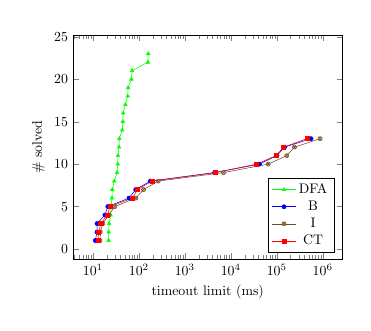
\begin{tikzpicture}[scale=0.5]
      \begin{axis}[
    xmode=log,
    every axis plot/.style={thin},
    xlabel={timeout limit (ms)},
    ylabel={\# solved},
    legend pos=south east
    % table/create on use/cumulative distribution/.style={
    %   create col/expr={\pgfmathaccuma + \thisrow{f(x)}}   
    % }
    ]
    \addplot 
    [mark=triangle*,
    mark size=1.5,
    mark options={solid},
    green] 
    coordinates {
    (21.989, 1)
(22.041, 2)
(22.559, 3)
(24.331, 4)
(24.974, 5)
(26.007, 6)
(26.462, 7)
(29.157, 8)
(33.602, 9)
(34.800, 10)
(35.158, 11)
(37.017, 12)
(37.604, 13)
(43.531, 14)
(44.847, 15)
(45.476, 16)
(50.917, 17)
(57.169, 18)
(58.349, 19)
(68.896, 20)
(71.202, 21)
(157.413, 22)
(159.802, 23)
    };

    \addplot 
    [blue,
    mark=*,
    mark size=1.5,
    mark options={solid}]
    coordinates {
    (11.281, 1)
(12.293, 2)
(12.323, 3)
(18.245, 4)
(21.125, 5)
(61.006, 6)
(85.311, 7)
(177.463, 8)
(4439.520, 9)
(41952.782, 10)
(100937.940, 11)
(147496.534, 12)
(556008.284, 13)
% (1000003.406, 14)
% (1000003.522, 15)
% (1000003.551, 16)
% (1000003.690, 17)
% (1000003.713, 18)
% (1000003.866, 19)
% (1000003.877, 20)
% (1000004.136, 21)
% (1000004.172, 22)
% (1000004.261, 23)
    };

    \addplot [brown!60!black,
    mark options={fill=brown!40},
    mark=otimes*,
    mark size=1.5]
    coordinates {
    (14.319, 1)
(14.525, 2)
(16.358, 3)
(22.251, 4)
(29.907, 5)
(86.300, 6)
(126.361, 7)
(264.396, 8)
(6937.110, 9)
(65105.320, 10)
(165084.246, 11)
(242777.983, 12)
(877449.095, 13)
% (1000004.285, 14)
% (1000004.482, 15)
% (1000004.500, 16)
% (1000004.632, 17)
% (1000004.858, 18)
% (1000004.869, 19)
% (1000004.994, 20)
% (1000015.307, 21)
% (1000021.218, 22)
% (1000094.474, 23)
    };

    \addplot 
    [red,
    mark size=1.5,
    mark=square*]
    coordinates {
    (12.839, 1)
(13.309, 2)
(14.887, 3)
(20.483, 4)
(23.742, 5)
(72.390, 6)
(93.185, 7)
(193.329, 8)
(4643.160, 9)
(36315.326, 10)
(96472.476, 11)
(140766.972, 12)
(452413.350, 13)
% (1000004.885, 14)
% (1000005.183, 15)
% (1000005.227, 16)
% (1000005.436, 17)
% (1000005.455, 18)
% (1000005.543, 19)
% (1000009.510, 20)
% (1000018.333, 21)
% (1000020.654, 22)
% (1000126.631, 23)
    };
    \legend{DFA,B,I,CT}
  \end{axis}

    \end{tikzpicture} \\
    
    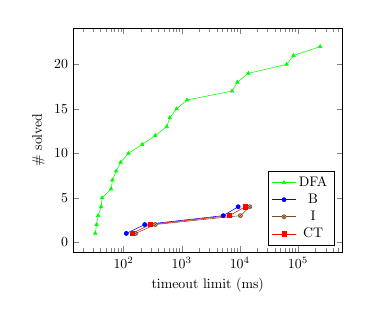
\begin{tikzpicture}[scale=0.5]
      \begin{axis}[
    xmode=log,
    every axis plot/.style={thin},
    xlabel={timeout limit (ms)},
    ylabel={\# solved},
    legend pos=south east
    % table/create on use/cumulative distribution/.style={
    %   create col/expr={\pgfmathaccuma + \thisrow{f(x)}}   
    % }
    ]
    \addplot 
    [mark=triangle*,
    mark size=1.5,
    mark options={solid},
    green] 
    coordinates {
    (32.646, 1)
(34.322, 2)
(36.539, 3)
(41.139, 4)
(42.637, 5)
(60.923, 6)
(64.362, 7)
(74.768, 8)
(89.108, 9)
(121.012, 10)
(208.525, 11)
(350.032, 12)
(553.291, 13)
(625.153, 14)
(813.725, 15)
(1234.205, 16)
(7361.018, 17)
(9076.992, 18)
(14005.709, 19)
(64038.325, 20)
(83738.459, 21)
(240798.763, 22)
    };

    \addplot 
    [blue,
    mark=*,
    mark size=1.5,
    mark options={solid}]
    coordinates {
    (111.532, 1)
(231.223, 2)
(5185.609, 3)
(9363.587, 4)
% (1000006.135, 5)
% (1000006.157, 6)
% (1000006.188, 7)
% (1000006.300, 8)
% (1000006.306, 9)
% (1000007.024, 10)
% (1000007.087, 11)
% (1000007.302, 12)
% (1000007.563, 13)
% (1000010.560, 14)
% (1000010.850, 15)
% (1000046.435, 16)
% (1000167.771, 17)
% (1001173.564, 18)
% (1006453.700, 19)
% (1008543.597, 20)
% (1010562.071, 21)
% (1019241.202, 22)
    };

    \addplot [brown!60!black,
    mark options={fill=brown!40},
    mark=otimes*,
    mark size=1.5]
    coordinates {
    (161.801, 1)
(350.376, 2)
(10244.105, 3)
(14856.666, 4)
% (1000007.483, 5)
% (1000007.625, 6)
% (1000007.695, 7)
% (1000008.729, 8)
% (1000009.950, 9)
% (1000011.262, 10)
% (1000019.536, 11)
% (1000023.192, 12)
% (1000025.767, 13)
% (1000040.365, 14)
% (1000041.636, 15)
% (1000051.012, 16)
% (1000053.849, 17)
% (1000118.768, 18)
% (1000166.508, 19)
% (1000467.387, 20)
% (1001776.595, 21)
% (1015356.678, 22)
    };

    \addplot 
    [red,
    mark size=1.5,
    mark=square*]
    coordinates {
    (140.045, 1)
(284.098, 2)
(6638.875, 3)
(12352.151, 4)
% (1000007.437, 5)
% (1000007.976, 6)
% (1000009.059, 7)
% (1000009.398, 8)
% (1000009.787, 9)
% (1000013.785, 10)
% (1000024.236, 11)
% (1000038.306, 12)
% (1000061.649, 13)
% (1000067.115, 14)
% (1000073.775, 15)
% (1000110.045, 16)
% (1000202.940, 17)
% (1000283.824, 18)
% (1001241.998, 19)
% (1012931.719, 20)
% (1016410.000, 21)
% (1021392.559, 22)
    };
    \legend{DFA,B,I,CT}
  \end{axis}

    \end{tikzpicture} & 
        \begin{tikzpicture}[scale=0.5]
      \begin{axis}[
    xmode=log,
    every axis plot/.style={thin},
    xlabel={timeout limit (ms)},
    ylabel={\% solved},
    legend pos=south east,
    cycle list/Set1-6,
            % define fill color for the marker
            mark list fill={.!75!white},
            mark options={solid},
            cycle multiindex* list={
                Set1-6
                    \nextlist
                [3 of]linestyles
                    \nextlist
                very thick
                \nextlist
                mark=o,
                mark=*,
                mark=square,
                mark=triangle,
                mark=+
            },
    ]

    \addplot
    coordinates {
      (221050, 50)
      
    };
    \addplot
    coordinates {
      (215740, 50)
      
    };
    \addplot
    coordinates {
      (286600, 50)
      
    };
    \addplot
    coordinates {
      (198370, 50)
      
    };
    

    \legend{ DFA, B, I, \textbf{CT} }
  \end{axis}

    \end{tikzpicture} \\

  \end{tabular}
\end{frame}

\begin{frame}
  \frametitle{Large tables}
  \framesubtitle{$2500-10000$~tuples}
  \begin{tabular}{cc}
    \begin{tikzpicture}[scale=0.5]
      \begin{axis}[
    xmode=log,
    every axis plot/.style={thin},
    xlabel={timeout limit (ms)},
    ylabel={\% solved},
    legend pos=south east,
    cycle list/Set1-6,
            % define fill color for the marker
            mark list fill={.!75!white},
            mark options={solid},
            cycle multiindex* list={
                Set1-6
                    \nextlist
                [3 of]linestyles
                    \nextlist
                very thick
                \nextlist
                mark=o,
                mark=*,
                mark=square,
                mark=triangle,
                mark=+
            },
    ]

    \addplot
    coordinates {
      (5500, 10)
      (16070, 20)
      (16630, 30)
      (17890, 40)
      (35390, 50)
      (57330, 60)
      (69990, 70)
      (101460, 80)
      (169980, 90)
      (453800, 100)
      
    };
    \addplot
    coordinates {
      (2230, 10)
      (5650, 20)
      (6980, 30)
      (8620, 40)
      (21360, 50)
      (25040, 60)
      (42030, 70)
      (56640, 80)
      (61450, 90)
      (253650, 100)
      
    };
    \addplot
    coordinates {
      (3120, 10)
      (9240, 20)
      (10460, 30)
      (12500, 40)
      (31710, 50)
      (38200, 60)
      (61930, 70)
      (82230, 80)
      (95830, 90)
      (382920, 100)
      
    };
    \addplot
    coordinates {
      (570, 10)
      (1250, 20)
      (1410, 30)
      (1570, 40)
      (3500, 50)
      (3990, 60)
      (6250, 70)
      (8860, 80)
      (10050, 90)
      (42870, 100)
      
    };
    

    \legend{ DFA, B, I, \textbf{CT} }
  \end{axis}

    \end{tikzpicture}
    &
      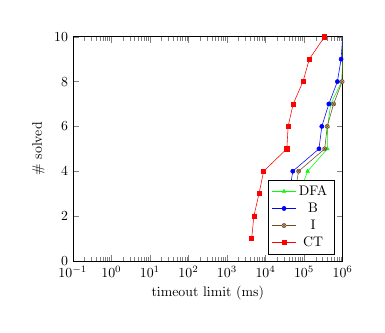
\begin{tikzpicture}[scale=0.5]
        \begin{axis}[
    xmode=log,
    ymin=0,ymax=10,
    xmin=0.1, xmax=1000000,
    every axis plot/.style={thin},
    xlabel={timeout limit (ms)},
    ylabel={\# solved},
    legend pos=south east
    % table/create on use/cumulative distribution/.style={
    %   create col/expr={\pgfmathaccuma + \thisrow{f(x)}}   
    % }
    ]
    \addplot 
    [mark=triangle*,
    mark size=1.5,
    mark options={solid},
    green] 
    coordinates {
    (37271.407, 1)
(63329.760, 2)
(75340.967, 3)
(123361.614, 4)
(400331.140, 5)
(406374.082, 6)
(491965.258, 7)
(943701.318, 8)
(1003127.715, 9)
(1003191.173, 10)
    };

    \addplot 
    [blue,
    mark=*,
    mark size=1.5,
    mark options={solid}]
    coordinates {
    (23487.263, 1)
(31493.067, 2)
(41324.456, 3)
(50843.172, 4)
(243499.863, 5)
(288078.384, 6)
(438078.025, 7)
(731291.713, 8)
(912991.209, 9)
(1000435.280, 10)
    };

    \addplot [brown!60!black,
    mark options={fill=brown!40},
    mark=otimes*,
    mark size=1.5]
    coordinates {
    (31721.470, 1)
(45760.945, 2)
(56699.417, 3)
(72142.510, 4)
(342690.713, 5)
(398501.909, 6)
(583027.925, 7)
(971126.357, 8)
(1000434.235, 9)
(1000435.846, 10)
    };

    \addplot 
    [red,
    mark size=1.5,
    mark=square*]
    coordinates {
    (4367.654, 1)
(4983.151, 2)
(6770.036, 3)
(8914.062, 4)
(35712.233, 5)
(38524.930, 6)
(52111.274, 7)
(93677.132, 8)
(136706.431, 9)
(338099.921, 10)
    };
    \legend{DFA,B,I,CT}
  \end{axis}

      \end{tikzpicture} \\
    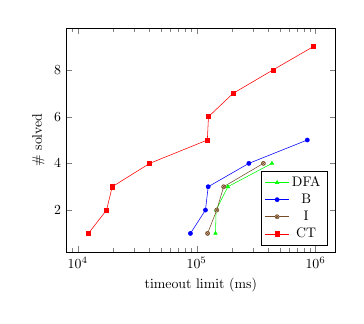
\begin{tikzpicture}[scale=0.5]
      \begin{axis}[
    xmode=log,
    every axis plot/.style={thin},
    xlabel={timeout limit (ms)},
    ylabel={\# solved},
    legend pos=south east
    % table/create on use/cumulative distribution/.style={
    %   create col/expr={\pgfmathaccuma + \thisrow{f(x)}}   
    % }
    ]
    \addplot 
    [mark=triangle*,
    mark size=1.5,
    mark options={solid},
    green] 
    coordinates {
    (143986.214, 1)
(145624.128, 2)
(182844.931, 3)
(429527.079, 4)
% (1004920.333, 5)
% (1005091.406, 6)
% (1005121.020, 7)
% (1005141.458, 8)
% (1005180.694, 9)
% (1005181.896, 10)
    };

    \addplot 
    [blue,
    mark=*,
    mark size=1.5,
    mark options={solid}]
    coordinates {
    (88610.730, 1)
(118513.380, 2)
(124991.902, 3)
(274645.919, 4)
(851285.302, 5)
% (1000662.235, 6)
% (1000665.157, 7)
% (1000667.124, 8)
% (1000679.084, 9)
% (1000680.879, 10)
    };

    \addplot [brown!60!black,
    mark options={fill=brown!40},
    mark=otimes*,
    mark size=1.5]
    coordinates {
    (123456.088, 1)
(147458.027, 2)
(168559.303, 3)
(363926.326, 4)
% (1000644.518, 5)
% (1000648.628, 6)
% (1000660.653, 7)
% (1000663.644, 8)
% (1000669.943, 9)
% (1000672.172, 10)
    };

    \addplot 
    [red,
    mark size=1.5,
    mark=square*]
    coordinates {
    (12283.482, 1)
(17462.103, 2)
(19503.895, 3)
(40266.047, 4)
(122893.209, 5)
(125673.584, 6)
(202682.066, 7)
(437565.193, 8)
(955387.007, 9)
%(1000911.643, 10)
    };
    \legend{DFA,B,I,CT}
  \end{axis}

    \end{tikzpicture}
    &
      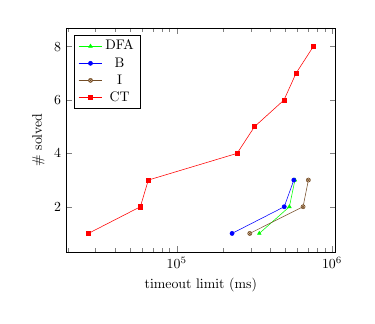
\begin{tikzpicture}[scale=0.5]
        \begin{axis}[
    xmode=log,
    every axis plot/.style={thin},
    xlabel={timeout limit (ms)},
    ylabel={\# solved},
    legend pos=north west
    % table/create on use/cumulative distribution/.style={
    %   create col/expr={\pgfmathaccuma + \thisrow{f(x)}}   
    % }
    ]
    \addplot 
    [mark=triangle*,
    mark size=1.5,
    mark options={solid},
    green] 
    coordinates {
    (339960.449, 1)
(531357.500, 2)
(576758.002, 3)
% (1006830.253, 4)
% (1006953.686, 5)
% (1006987.278, 6)
% (1007012.182, 7)
% (1007040.479, 8)
% (1007166.422, 9)
% (1007385.382, 10)
    };

    \addplot 
    [blue,
    mark=*,
    mark size=1.5,
    mark options={solid}]
    coordinates {
    (227052.199, 1)
(492242.811, 2)
(567372.313, 3)
% (1000877.234, 4)
% (1000889.042, 5)
% (1000892.874, 6)
% (1000895.207, 7)
% (1000911.856, 8)
% (1000913.878, 9)
% (1000928.789, 10)
    };

    \addplot [brown!60!black,
    mark options={fill=brown!40},
    mark=otimes*,
    mark size=1.5]
    coordinates {
    (295287.152, 1)
(650810.991, 2)
(703794.608, 3)
% (1000887.426, 4)
% (1000895.815, 5)
% (1000897.600, 6)
% (1000901.551, 7)
% (1000905.923, 8)
% (1000907.888, 9)
% (1000913.436, 10)
    };

    \addplot 
    [red,
    mark size=1.5,
    mark=square*]
    coordinates {
    (26984.703, 1)
(58304.179, 2)
(65624.179, 3)
(244616.117, 4)
(316746.918, 5)
(490346.243, 6)
(586068.768, 7)
(756641.057, 8)
%(1001171.576, 9)
%(1001192.839, 10)
    };
    \legend{DFA,B,I,CT}
  \end{axis}

      \end{tikzpicture} \\
  \end{tabular}
\end{frame}

\begin{frame}
  \frametitle{Large tables}
  \framesubtitle{$> 12000$~tuples}
  \begin{tabular}{cc}
    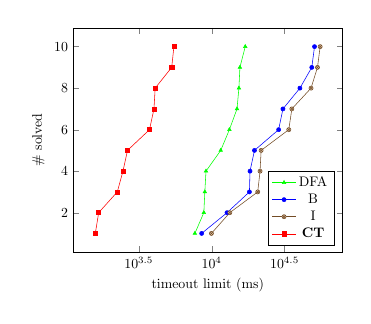
\begin{tikzpicture}[scale=0.5]
      \begin{axis}[
    xmode=log,
    every axis plot/.style={thin},
    xlabel={timeout limit (ms)},
    ylabel={\# solved},
    legend pos=south east
    % table/create on use/cumulative distribution/.style={
    %   create col/expr={\pgfmathaccuma + \thisrow{f(x)}}   
    % }
    ]
    \addplot 
    [mark=triangle*,
    mark size=1.5,
    mark options={solid},
    green] 
    coordinates {
    (7669.883, 1)
(8836.338, 2)
(8977.330, 3)
(9140.777, 4)
(11537.562, 5)
(13231.384, 6)
(14923.762, 7)
(15381.136, 8)
(15623.402, 9)
(16994.255, 10)
    };

    \addplot 
    [blue,
    mark=*,
    mark size=1.5,
    mark options={solid}]
    coordinates {
    (8538.228, 1)
(12749.685, 2)
(18156.956, 3)
(18327.323, 4)
(19669.292, 5)
(28802.590, 6)
(30835.715, 7)
(40301.654, 8)
(48620.995, 9)
(50774.009, 10)
    };

    \addplot [brown!60!black,
    mark options={fill=brown!40},
    mark=otimes*,
    mark size=1.5]
    coordinates {
    (9960.047, 1)
(13326.927, 2)
(20700.530, 3)
(21474.840, 4)
(21842.271, 5)
(33817.893, 6)
(35489.987, 7)
(48049.593, 8)
(53196.297, 9)
(55499.785, 10)
    };

    \addplot 
    [red,
    mark size=1.5,
    mark=square*]
    coordinates {
    (1591.239, 1)
(1678.457, 2)
(2251.773, 3)
(2462.919, 4)
(2646.514, 5)
(3745.993, 6)
(4020.526, 7)
(4095.836, 8)
(5320.617, 9)
(5507.353, 10)
    };
    \legend{DFA,B,I,\textbf{CT}}
  \end{axis}

    \end{tikzpicture}
    &
      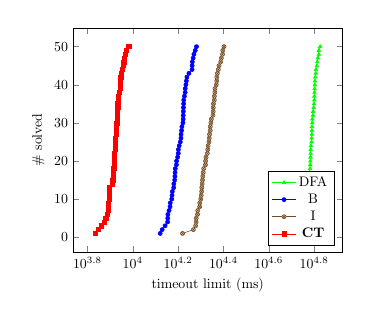
\begin{tikzpicture}[scale=0.5]
        \begin{axis}[
    xmode=log,
    every axis plot/.style={thin},
    xlabel={timeout limit (ms)},
    ylabel={\# solved},
    legend pos=south east
    % table/create on use/cumulative distribution/.style={
    %   create col/expr={\pgfmathaccuma + \thisrow{f(x)}}   
    % }
    ]
    \addplot 
    [mark=triangle*,
    mark size=1.5,
    mark options={solid},
    green] 
    coordinates {
    (51125.785, 1)
(54263.257, 2)
(56487.527, 3)
(56702.786, 4)
(56985.792, 5)
(57276.885, 6)
(57622.584, 7)
(58132.270, 8)
(58140.300, 9)
(58355.175, 10)
(58676.203, 11)
(59158.883, 12)
(59632.816, 13)
(59713.900, 14)
(59728.215, 15)
(60269.934, 16)
(60313.648, 17)
(60549.505, 18)
(60622.637, 19)
(60711.449, 20)
(60810.980, 21)
(60862.784, 22)
(60914.293, 23)
(61100.454, 24)
(61428.994, 25)
(61523.477, 26)
(61625.366, 27)
(61712.915, 28)
(61729.236, 29)
(61886.596, 30)
(61900.845, 31)
(62341.893, 32)
(62455.546, 33)
(62817.572, 34)
(63010.646, 35)
(63184.232, 36)
(63221.376, 37)
(63304.994, 38)
(63379.424, 39)
(63540.272, 40)
(63613.419, 41)
(63781.589, 42)
(64128.455, 43)
(64263.902, 44)
(64924.220, 45)
(65113.900, 46)
(65508.695, 47)
(66133.866, 48)
(66157.482, 49)
(67076.860, 50)
    };

    \addplot 
    [blue,
    mark=*,
    mark size=1.5,
    mark options={solid}]
    coordinates {
    (13210.645, 1)
(13478.699, 2)
(13880.904, 3)
(14240.906, 4)
(14262.586, 5)
(14281.012, 6)
(14453.879, 7)
(14601.257, 8)
(14630.915, 9)
(14856.229, 10)
(14906.587, 11)
(14947.426, 12)
(15147.432, 13)
(15173.599, 14)
(15300.351, 15)
(15338.350, 16)
(15370.471, 17)
(15400.162, 18)
(15575.398, 19)
(15599.555, 20)
(15767.367, 21)
(15876.487, 22)
(15890.540, 23)
(16026.936, 24)
(16207.081, 25)
(16313.213, 26)
(16328.178, 27)
(16410.911, 28)
(16468.425, 29)
(16641.910, 30)
(16678.794, 31)
(16689.212, 32)
(16716.749, 33)
(16728.322, 34)
(16755.929, 35)
(16780.814, 36)
(16896.779, 37)
(17026.619, 38)
(17037.921, 39)
(17147.387, 40)
(17237.324, 41)
(17326.549, 42)
(17685.575, 43)
(18266.956, 44)
(18281.157, 45)
(18310.293, 46)
(18466.165, 47)
(18608.783, 48)
(18864.433, 49)
(19102.683, 50)
    };

    \addplot [brown!60!black,
    mark options={fill=brown!40},
    mark=otimes*,
    mark size=1.5]
    coordinates {
    (16575.843, 1)
(18505.000, 2)
(18940.008, 3)
(19038.980, 4)
(19049.304, 5)
(19298.221, 6)
(19348.596, 7)
(19719.698, 8)
(19737.753, 9)
(19947.661, 10)
(20036.932, 11)
(20122.714, 12)
(20152.397, 13)
(20232.116, 14)
(20302.198, 15)
(20360.843, 16)
(20458.853, 17)
(20543.247, 18)
(20924.864, 19)
(20941.580, 20)
(21033.055, 21)
(21323.434, 22)
(21424.912, 23)
(21488.205, 24)
(21690.524, 25)
(21732.563, 26)
(21805.424, 27)
(21961.943, 28)
(21968.175, 29)
(22103.640, 30)
(22217.515, 31)
(22576.655, 32)
(22629.332, 33)
(22640.426, 34)
(22690.290, 35)
(22898.044, 36)
(22906.588, 37)
(23018.632, 38)
(23049.661, 39)
(23346.986, 40)
(23464.371, 41)
(23482.242, 42)
(23611.320, 43)
(23844.593, 44)
(24011.531, 45)
(24420.146, 46)
(24590.635, 47)
(24882.878, 48)
(24954.062, 49)
(25252.813, 50)
    };

    \addplot 
    [red,
    mark size=1.5,
    mark=square*]
    coordinates {
    (6834.272, 1)
(7049.566, 2)
(7238.120, 3)
(7457.754, 4)
(7598.772, 5)
(7739.737, 6)
(7771.586, 7)
(7772.970, 8)
(7812.433, 9)
(7861.439, 10)
(7862.003, 11)
(7867.552, 12)
(7871.233, 13)
(8146.006, 14)
(8162.853, 15)
(8169.022, 16)
(8197.217, 17)
(8246.900, 18)
(8258.157, 19)
(8262.374, 20)
(8291.516, 21)
(8318.251, 22)
(8342.451, 23)
(8355.561, 24)
(8389.425, 25)
(8401.690, 26)
(8470.665, 27)
(8475.034, 28)
(8489.871, 29)
(8495.761, 30)
(8507.506, 31)
(8510.152, 32)
(8560.945, 33)
(8587.622, 34)
(8588.072, 35)
(8642.789, 36)
(8662.209, 37)
(8738.285, 38)
(8798.802, 39)
(8820.422, 40)
(8831.432, 41)
(8851.771, 42)
(8928.438, 43)
(8949.293, 44)
(9107.856, 45)
(9118.812, 46)
(9135.516, 47)
(9225.896, 48)
(9370.806, 49)
(9607.234, 50)
    };
    \legend{DFA,B,I,\textbf{CT}}
  \end{axis}

      \end{tikzpicture} \\
    \begin{tikzpicture}[scale=0.5]
      \begin{axis}[
    xmode=log,
    every axis plot/.style={thin},
    xlabel={timeout limit (ms)},
    ylabel={\% solved},
    legend style={at={(0.5,-0.30)},
      anchor=north,legend columns=-1},
    % legend pos=south east,
    cycle list/Set1-6,
            % define fill color for the marker
            mark list fill={.!75!white},
            mark options={solid,scale=0.9},
            cycle multiindex* list={
                Set1-6
                    \nextlist
                [3 of]linestyles
                    \nextlist
                very thick
                \nextlist
                mark=o,
                mark=*,
                mark=square,
                mark=triangle,
                mark=+
            },
    ]

    \addplot
    coordinates {

    };
    \addplot
    coordinates {
      (218870, 2)
      (301170, 4)
      (482210, 6)
      (553150, 8)
      (794860, 10)

    };
    \addplot
    coordinates {
      (296190, 2)
      (404230, 4)
      (606290, 6)
      (680520, 8)

    };
    \addplot
    coordinates {
      (15250, 2)
      (31320, 4)
      (36930, 6)
      (44950, 8)
      (48590, 10)
      (84800, 12)
      (105320, 15)
      (122290, 16)
      (149390, 18)
      (190110, 20)
      (199080, 22)
      (203260, 24)
      (205030, 26)
      (294700, 29)
      (410490, 30)
      (517330, 32)
      (796770, 34)

    };


    \legend{ B, I, \textbf{CT} }
  \end{axis}

    \end{tikzpicture}
    &
      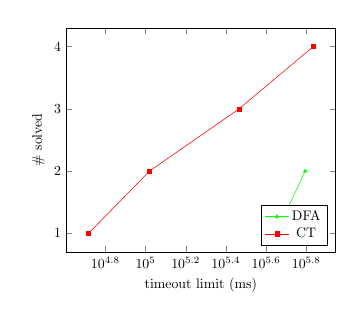
\begin{tikzpicture}[scale=0.5]
        \begin{axis}[
    xmode=log,
    every axis plot/.style={thin},
    xlabel={timeout limit (ms)},
    ylabel={\# solved},
    legend pos=south east
    % table/create on use/cumulative distribution/.style={
    %   create col/expr={\pgfmathaccuma + \thisrow{f(x)}}   
    % }
    ]
    \addplot 
    [mark=triangle*,
    mark size=1.5,
    mark options={solid},
    green] 
    coordinates {
    (445273.296, 1)
(622414.790, 2)
% (1031281.648, 3)
% (1073752.509, 4)
% (1077338.303, 5)
% (1078117.880, 6)
% (1078636.961, 7)
% (1079178.894, 8)
% (1079839.216, 9)
% (1080840.349, 10)
% (1082059.397, 11)
% (1083648.155, 12)
% (1083902.339, 13)
% (1083988.269, 14)
% (1084069.534, 15)
% (1084396.676, 16)
% (1085666.524, 17)
% (1089495.967, 18)
% (1091132.921, 19)
% (1091433.340, 20)
% (1092057.252, 21)
% (1093916.092, 22)
% (1094177.223, 23)
% (1114453.122, 24)
% (1115067.373, 25)
    };

%     \addplot 
%     [blue,
%     mark=*,
%     mark size=1.5,
%     mark options={solid}]
%     coordinates {
%     (1004672.786, 1)
% (1004695.224, 2)
% (1004696.645, 3)
% (1004718.463, 4)
% (1004738.023, 5)
% (1004743.967, 6)
% (1004751.151, 7)
% (1004765.567, 8)
% (1004781.515, 9)
% (1004797.803, 10)
% (1004816.640, 11)
% (1004820.096, 12)
% (1004835.673, 13)
% (1004864.792, 14)
% (1004881.537, 15)
% (1004913.526, 16)
% (1004920.059, 17)
% (1004929.625, 18)
% (1004958.448, 19)
% (1004996.508, 20)
% (1005007.752, 21)
% (1005029.139, 22)
% (1005067.535, 23)
% (1005104.606, 24)
% (1040982.750, 25)
%     };

%     \addplot [brown!60!black,
%     mark options={fill=brown!40},
%     mark=otimes*,
%     mark size=1.5]
%     coordinates {
%     (1004653.569, 1)
% (1004695.464, 2)
% (1004715.665, 3)
% (1004725.629, 4)
% (1004729.598, 5)
% (1004736.757, 6)
% (1004768.906, 7)
% (1004774.513, 8)
% (1004800.095, 9)
% (1004877.671, 10)
% (1004885.444, 11)
% (1004924.289, 12)
% (1004954.273, 13)
% (1004976.220, 14)
% (1005012.748, 15)
% (1005016.479, 16)
% (1005025.501, 17)
% (1005059.309, 18)
% (1005081.774, 19)
% (1005131.686, 20)
% (1005177.022, 21)
% (1005199.107, 22)
% (1005247.884, 23)
% (1005272.462, 24)
% (1103825.908, 25)
%     };

    \addplot 
    [red,
    mark size=1.5,
    mark=square*]
    coordinates {
    (51933.780, 1)
(104573.439, 2)
(291800.057, 3)
(683133.039, 4)
% (1006259.610, 5)
% (1006270.822, 6)
% (1006282.419, 7)
% (1006303.104, 8)
% (1006319.339, 9)
% (1006423.422, 10)
% (1006449.607, 11)
% (1006459.928, 12)
% (1006499.500, 13)
% (1006510.783, 14)
% (1006510.952, 15)
% (1006511.373, 16)
% (1006567.036, 17)
% (1006579.356, 18)
% (1006588.135, 19)
% (1006591.883, 20)
% (1006659.196, 21)
% (1006817.280, 22)
% (1006986.645, 23)
% (1012355.582, 24)
% (1025624.781, 25)
    };
    \legend{DFA,CT}
  \end{axis}

      \end{tikzpicture} \\
  \end{tabular}
\end{frame}

\begin{frame}
  \frametitle{Low arities}
  \framesubtitle{$2-3$~variables}
  \begin{tabular}{cc}
    \begin{tikzpicture}[scale=0.5]
      \begin{axis}[
    xmode=log,
    every axis plot/.style={thin},
    xlabel={timeout limit (ms)},
    ylabel={\% solved},
    legend pos=south east,
    cycle list/Set1-6,
            % define fill color for the marker
            mark list fill={.!75!white},
            mark options={solid},
            cycle multiindex* list={
                Set1-6
                    \nextlist
                [3 of]linestyles
                    \nextlist
                very thick
                \nextlist
                mark=o,
                mark=*,
                mark=square,
                mark=triangle,
                mark=+
            },
    ]

    \addplot
    coordinates {
      (1410, 20)
      (2980, 40)
      (7950, 60)
      (22760, 80)
      (78820, 100)
      
    };
    \addplot
    coordinates {
      (650, 20)
      (1930, 40)
      (7810, 60)
      (29790, 80)
      (124670, 100)
      
    };
    \addplot
    coordinates {
      (740, 20)
      (2300, 40)
      (9460, 60)
      (36010, 80)
      (148310, 100)
      
    };
    \addplot
    coordinates {
      (580, 20)
      (1530, 40)
      (5640, 60)
      (20620, 80)
      (82360, 100)
      
    };
    

    \legend{ DFA, B, I, \textbf{CT} }
  \end{axis}

    \end{tikzpicture}
    &
      \begin{tikzpicture}[scale=0.5]
        \begin{axis}[
    xmode=log,
    every axis plot/.style={thin},
    xlabel={timeout limit (ms)},
    ylabel={\% solved},
    legend pos=south east,
    cycle list/Set1-6,
            % define fill color for the marker
            mark list fill={.!75!white},
            mark options={solid},
            cycle multiindex* list={
                Set1-6
                    \nextlist
                [3 of]linestyles
                    \nextlist
                very thick
                \nextlist
                mark=o,
                mark=*,
                mark=square,
                mark=triangle,
                mark=+
            },
    ]

    \addplot
    coordinates {
      (221050, 50)
      
    };
    \addplot
    coordinates {
      (215740, 50)
      
    };
    \addplot
    coordinates {
      (286600, 50)
      
    };
    \addplot
    coordinates {
      (198370, 50)
      
    };
    

    \legend{ DFA, B, I, \textbf{CT} }
  \end{axis}

      \end{tikzpicture} \\
    \begin{tikzpicture}[scale=0.5]
      \begin{axis}[
    xmode=log,
    every axis plot/.style={thin},
    xlabel={timeout limit (ms)},
    ylabel={\% solved},
    legend style={at={(0.5,-0.30)},
      anchor=north,legend columns=-1},
    % legend pos=south east,
    cycle list/Set1-6,
            % define fill color for the marker
            mark list fill={.!75!white},
            mark options={solid,scale=0.9},
            cycle multiindex* list={
                Set1-6
                    \nextlist
                [3 of]linestyles
                    \nextlist
                very thick
                \nextlist
                mark=o,
                mark=*,
                mark=square,
                mark=triangle,
                mark=+
            },
    ]

    \addplot
    coordinates {
      (550, 7)
      (1420, 13)
      (2180, 19)
      (2460, 25)
      (4050, 32)
      (11860, 38)
      (37590, 44)
      (42030, 50)
      (51040, 57)
      (744510, 63)
      (828510, 69)
      (921350, 75)
      
    };
    \addplot
    coordinates {
      (730, 7)
      (2790, 13)
      (2950, 19)
      (9950, 25)
      (22390, 32)
      (55820, 38)
      (79890, 44)
      (247070, 50)
      
    };
    \addplot
    coordinates {
      (720, 7)
      (2880, 13)
      (4460, 19)
      (11570, 25)
      (21880, 32)
      (80590, 38)
      (84470, 44)
      (276470, 50)
      
    };
    \addplot
    coordinates {
      (140, 7)
      (210, 13)
      (680, 19)
      (1410, 25)
      (1760, 32)
      (2610, 38)
      (23590, 44)
      (29830, 50)
      (49050, 57)
      (474090, 63)
      (606460, 69)
      
    };
    

    \legend{ DFA, B, I, \textbf{CT} }
  \end{axis}

    \end{tikzpicture}
    &
      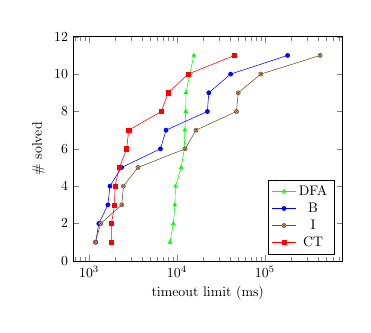
\begin{tikzpicture}[scale=0.5]
        \begin{axis}[
    xmode=log,
    every axis plot/.style={thin},
    xlabel={timeout limit (ms)},
    ylabel={\# solved},
    legend pos=south east
    % table/create on use/cumulative distribution/.style={
    %   create col/expr={\pgfmathaccuma + \thisrow{f(x)}}   
    % }
    ]
    \addplot 
    [mark=triangle*,
    mark size=1.5,
    mark options={solid},
    green] 
    coordinates {
    (8323.942, 1)
(9080.418, 2)
(9457.327, 3)
(9611.154, 4)
(11157.909, 5)
(12122.318, 6)
(12269.578, 7)
(12569.631, 8)
(12613.425, 9)
(13987.860, 10)
(15538.867, 11)
    };

    \addplot 
    [blue,
    mark=*,
    mark size=1.5,
    mark options={solid}]
    coordinates {
    (1188.206, 1)
(1289.021, 2)
(1636.318, 3)
(1725.962, 4)
(2339.887, 5)
(6481.991, 6)
(7504.933, 7)
(22155.924, 8)
(23009.793, 9)
(40756.444, 10)
(181399.438, 11)
    };

    \addplot [brown!60!black,
    mark options={fill=brown!40},
    mark=otimes*,
    mark size=1.5]
    coordinates {
    (1175.718, 1)
(1354.438, 2)
(2353.159, 3)
(2454.453, 4)
(3594.396, 5)
(12379.752, 6)
(16444.353, 7)
(47478.184, 8)
(49773.525, 9)
(89852.322, 10)
(425399.368, 11)
    };

    \addplot 
    [red,
    mark size=1.5,
    mark=square*]
    coordinates {
    (1794.640, 1)
(1795.355, 2)
(1951.150, 3)
(1965.074, 4)
(2212.001, 5)
(2673.018, 6)
(2822.171, 7)
(6633.134, 8)
(7933.220, 9)
(13389.469, 10)
(45079.672, 11)
    };
    \legend{DFA,B,I,CT}
  \end{axis}

      \end{tikzpicture} \\
  \end{tabular}
\end{frame}

\begin{frame}
  \frametitle{High arities}
  \framesubtitle{$>5$~variables}
  \begin{tabular}{cc}
    \begin{tikzpicture}[scale=0.5]
      \begin{axis}[
    xmode=log,
    every axis plot/.style={thin},
    xlabel={timeout limit (ms)},
    ylabel={\% solved},
    legend pos=south east,
    cycle list/Set1-6,
            % define fill color for the marker
            mark list fill={.!75!white},
            mark options={solid},
            cycle multiindex* list={
                Set1-6
                    \nextlist
                [3 of]linestyles
                    \nextlist
                very thick
                \nextlist
                mark=o,
                mark=*,
                mark=square,
                mark=triangle,
                mark=+
            },
    ]

    \addplot
    coordinates {
      (663310, 3)
      (668120, 6)
      (674240, 9)
      (681210, 12)
      (682080, 15)
      (693360, 18)
      (701800, 20)
      (710510, 23)
      (721370, 26)
      (733270, 29)
      (737690, 32)
      (743100, 35)
      (744950, 38)
      (746390, 40)
      (747580, 43)
      (747780, 46)
      (749520, 49)
      (752380, 52)
      (752460, 55)
      (752970, 58)
      (756240, 60)
      (756590, 63)
      (757070, 66)
      (757940, 69)
      (757950, 72)
      (758210, 75)
      (760950, 78)
      (761150, 80)
      (761270, 83)
      (762350, 86)
      (764150, 89)
      (764630, 92)
      (766660, 95)
      (778590, 98)
      (779820, 100)
      
    };
    \addplot
    coordinates {
      (48960, 3)
      (50130, 6)
      (50220, 9)
      (51730, 12)
      (52950, 15)
      (53810, 18)
      (78780, 20)
      (117310, 23)
      (204580, 26)
      (211480, 29)
      (211610, 32)
      (214100, 35)
      (218950, 38)
      (219710, 40)
      (221560, 43)
      (223130, 46)
      (225000, 49)
      (225250, 52)
      (226390, 55)
      (228770, 58)
      (228800, 60)
      (229210, 63)
      (229280, 66)
      (230400, 69)
      (230980, 72)
      (232150, 78)
      (236310, 80)
      (236880, 83)
      (237290, 86)
      (237320, 89)
      (238430, 92)
      (242000, 95)
      (247080, 98)
      (259880, 100)
      
    };
    \addplot
    coordinates {
      (48610, 3)
      (49700, 6)
      (49990, 9)
      (50810, 12)
      (51050, 15)
      (53250, 18)
      (90540, 20)
      (142650, 23)
      (275900, 26)
      (280260, 29)
      (282090, 32)
      (283200, 35)
      (283420, 38)
      (285910, 40)
      (287700, 43)
      (288220, 46)
      (291090, 49)
      (291560, 52)
      (294120, 55)
      (297560, 58)
      (297750, 60)
      (299160, 63)
      (300220, 66)
      (300620, 69)
      (301270, 72)
      (304330, 75)
      (308970, 78)
      (310620, 80)
      (310750, 83)
      (310990, 86)
      (311140, 89)
      (315640, 92)
      (328920, 95)
      (329910, 98)
      (341360, 100)
      
    };
    \addplot
    coordinates {
      (53490, 3)
      (54330, 6)
      (54840, 9)
      (55390, 12)
      (55780, 15)
      (56350, 18)
      (62080, 20)
      (76760, 23)
      (89920, 26)
      (92730, 29)
      (93300, 32)
      (93750, 35)
      (93760, 38)
      (93770, 40)
      (93910, 43)
      (94080, 46)
      (94190, 49)
      (94750, 52)
      (95060, 55)
      (95240, 58)
      (95480, 60)
      (95620, 63)
      (95790, 66)
      (95950, 69)
      (96350, 72)
      (96460, 78)
      (97070, 80)
      (97530, 83)
      (98260, 86)
      (98700, 89)
      (99170, 92)
      (99350, 95)
      (99830, 98)
      (100100, 100)
      
    };
    

    \legend{ DFA, B, I, \textbf{CT} }
  \end{axis}

    \end{tikzpicture}
    &
      \begin{tikzpicture}[scale=0.5]
        \begin{axis}[
    xmode=log,
    every axis plot/.style={thin},
    xlabel={timeout limit (ms)},
    ylabel={\% solved},
    legend style={at={(0.5,-0.30)},
      anchor=north,legend columns=-1},
    % legend pos=south east,
    cycle list/Set1-6,
            % define fill color for the marker
            mark list fill={.!75!white},
            mark options={solid,scale=0.9},
            cycle multiindex* list={
                Set1-6
                    \nextlist
                [3 of]linestyles
                    \nextlist
                very thick
                \nextlist
                mark=o,
                mark=*,
                mark=square,
                mark=triangle,
                mark=+
            },
    ]

    \addplot
    coordinates {
      (1070, 3)
      (1090, 6)
      (1100, 9)
      (1140, 12)
      (1340, 15)
      (1620, 18)
      (1650, 20)
      (1780, 23)
      (1830, 26)
      (2280, 29)
      (2300, 32)
      (2340, 35)
      (2490, 38)
      (2750, 40)
      (2880, 43)
      (3070, 46)
      (3780, 49)
      (3960, 52)
      (4590, 55)
      (4680, 58)
      (4980, 60)
      (5180, 63)
      (5480, 66)
      (8310, 69)
      (11060, 72)
      (11440, 75)
      (14310, 78)
      (15080, 80)
      (23840, 83)
      (28160, 86)
      (34450, 89)
      (35060, 92)
      (45870, 95)
      (49120, 98)
      (62030, 100)
      
    };
    \addplot
    coordinates {
      (50, 6)
      (60, 9)
      (70, 12)
      (80, 18)
      (130, 23)
      (200, 26)
      (240, 29)
      (330, 32)
      (360, 35)
      (840, 38)
      (1000, 40)
      (1340, 43)
      (1420, 46)
      (1570, 49)
      (2440, 52)
      (2810, 55)
      (4430, 58)
      (5330, 60)
      (7350, 63)
      (7450, 66)
      (12850, 69)
      (16490, 72)
      (19310, 75)
      (20520, 78)
      (23670, 80)
      (39020, 83)
      (62930, 86)
      (65710, 89)
      (70870, 92)
      (109260, 95)
      (117110, 98)
      (144570, 100)
      
    };
    \addplot
    coordinates {
      (50, 6)
      (70, 12)
      (100, 18)
      (170, 20)
      (190, 23)
      (300, 26)
      (320, 29)
      (500, 35)
      (1120, 38)
      (1330, 40)
      (1630, 43)
      (1720, 46)
      (2180, 49)
      (3200, 52)
      (3680, 55)
      (5710, 58)
      (6810, 60)
      (9230, 63)
      (9390, 66)
      (16190, 69)
      (18960, 72)
      (24090, 75)
      (25580, 78)
      (29300, 80)
      (47970, 83)
      (75460, 86)
      (80010, 89)
      (85710, 92)
      (129810, 95)
      (138470, 98)
      (170370, 100)
      
    };
    \addplot
    coordinates {
      (50, 6)
      (60, 9)
      (70, 12)
      (80, 18)
      (100, 20)
      (110, 26)
      (140, 29)
      (160, 32)
      (180, 35)
      (230, 38)
      (240, 40)
      (260, 43)
      (300, 46)
      (440, 49)
      (520, 52)
      (580, 55)
      (820, 58)
      (970, 60)
      (1270, 63)
      (1290, 66)
      (2040, 69)
      (2350, 72)
      (3050, 75)
      (3340, 78)
      (3870, 80)
      (6030, 83)
      (10650, 86)
      (10890, 89)
      (11130, 92)
      (14780, 95)
      (20090, 98)
      (24080, 100)
      
    };
    

    \legend{ DFA, B, I, \textbf{CT} }
  \end{axis}

      \end{tikzpicture} \\
    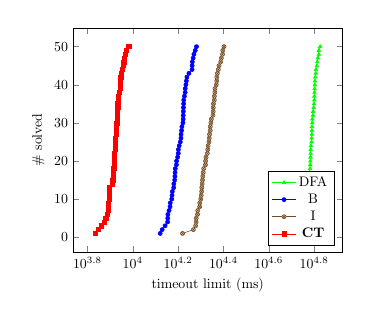
\begin{tikzpicture}[scale=0.5]
      \begin{axis}[
    xmode=log,
    every axis plot/.style={thin},
    xlabel={timeout limit (ms)},
    ylabel={\# solved},
    legend pos=south east
    % table/create on use/cumulative distribution/.style={
    %   create col/expr={\pgfmathaccuma + \thisrow{f(x)}}   
    % }
    ]
    \addplot 
    [mark=triangle*,
    mark size=1.5,
    mark options={solid},
    green] 
    coordinates {
    (51125.785, 1)
(54263.257, 2)
(56487.527, 3)
(56702.786, 4)
(56985.792, 5)
(57276.885, 6)
(57622.584, 7)
(58132.270, 8)
(58140.300, 9)
(58355.175, 10)
(58676.203, 11)
(59158.883, 12)
(59632.816, 13)
(59713.900, 14)
(59728.215, 15)
(60269.934, 16)
(60313.648, 17)
(60549.505, 18)
(60622.637, 19)
(60711.449, 20)
(60810.980, 21)
(60862.784, 22)
(60914.293, 23)
(61100.454, 24)
(61428.994, 25)
(61523.477, 26)
(61625.366, 27)
(61712.915, 28)
(61729.236, 29)
(61886.596, 30)
(61900.845, 31)
(62341.893, 32)
(62455.546, 33)
(62817.572, 34)
(63010.646, 35)
(63184.232, 36)
(63221.376, 37)
(63304.994, 38)
(63379.424, 39)
(63540.272, 40)
(63613.419, 41)
(63781.589, 42)
(64128.455, 43)
(64263.902, 44)
(64924.220, 45)
(65113.900, 46)
(65508.695, 47)
(66133.866, 48)
(66157.482, 49)
(67076.860, 50)
    };

    \addplot 
    [blue,
    mark=*,
    mark size=1.5,
    mark options={solid}]
    coordinates {
    (13210.645, 1)
(13478.699, 2)
(13880.904, 3)
(14240.906, 4)
(14262.586, 5)
(14281.012, 6)
(14453.879, 7)
(14601.257, 8)
(14630.915, 9)
(14856.229, 10)
(14906.587, 11)
(14947.426, 12)
(15147.432, 13)
(15173.599, 14)
(15300.351, 15)
(15338.350, 16)
(15370.471, 17)
(15400.162, 18)
(15575.398, 19)
(15599.555, 20)
(15767.367, 21)
(15876.487, 22)
(15890.540, 23)
(16026.936, 24)
(16207.081, 25)
(16313.213, 26)
(16328.178, 27)
(16410.911, 28)
(16468.425, 29)
(16641.910, 30)
(16678.794, 31)
(16689.212, 32)
(16716.749, 33)
(16728.322, 34)
(16755.929, 35)
(16780.814, 36)
(16896.779, 37)
(17026.619, 38)
(17037.921, 39)
(17147.387, 40)
(17237.324, 41)
(17326.549, 42)
(17685.575, 43)
(18266.956, 44)
(18281.157, 45)
(18310.293, 46)
(18466.165, 47)
(18608.783, 48)
(18864.433, 49)
(19102.683, 50)
    };

    \addplot [brown!60!black,
    mark options={fill=brown!40},
    mark=otimes*,
    mark size=1.5]
    coordinates {
    (16575.843, 1)
(18505.000, 2)
(18940.008, 3)
(19038.980, 4)
(19049.304, 5)
(19298.221, 6)
(19348.596, 7)
(19719.698, 8)
(19737.753, 9)
(19947.661, 10)
(20036.932, 11)
(20122.714, 12)
(20152.397, 13)
(20232.116, 14)
(20302.198, 15)
(20360.843, 16)
(20458.853, 17)
(20543.247, 18)
(20924.864, 19)
(20941.580, 20)
(21033.055, 21)
(21323.434, 22)
(21424.912, 23)
(21488.205, 24)
(21690.524, 25)
(21732.563, 26)
(21805.424, 27)
(21961.943, 28)
(21968.175, 29)
(22103.640, 30)
(22217.515, 31)
(22576.655, 32)
(22629.332, 33)
(22640.426, 34)
(22690.290, 35)
(22898.044, 36)
(22906.588, 37)
(23018.632, 38)
(23049.661, 39)
(23346.986, 40)
(23464.371, 41)
(23482.242, 42)
(23611.320, 43)
(23844.593, 44)
(24011.531, 45)
(24420.146, 46)
(24590.635, 47)
(24882.878, 48)
(24954.062, 49)
(25252.813, 50)
    };

    \addplot 
    [red,
    mark size=1.5,
    mark=square*]
    coordinates {
    (6834.272, 1)
(7049.566, 2)
(7238.120, 3)
(7457.754, 4)
(7598.772, 5)
(7739.737, 6)
(7771.586, 7)
(7772.970, 8)
(7812.433, 9)
(7861.439, 10)
(7862.003, 11)
(7867.552, 12)
(7871.233, 13)
(8146.006, 14)
(8162.853, 15)
(8169.022, 16)
(8197.217, 17)
(8246.900, 18)
(8258.157, 19)
(8262.374, 20)
(8291.516, 21)
(8318.251, 22)
(8342.451, 23)
(8355.561, 24)
(8389.425, 25)
(8401.690, 26)
(8470.665, 27)
(8475.034, 28)
(8489.871, 29)
(8495.761, 30)
(8507.506, 31)
(8510.152, 32)
(8560.945, 33)
(8587.622, 34)
(8588.072, 35)
(8642.789, 36)
(8662.209, 37)
(8738.285, 38)
(8798.802, 39)
(8820.422, 40)
(8831.432, 41)
(8851.771, 42)
(8928.438, 43)
(8949.293, 44)
(9107.856, 45)
(9118.812, 46)
(9135.516, 47)
(9225.896, 48)
(9370.806, 49)
(9607.234, 50)
    };
    \legend{DFA,B,I,\textbf{CT}}
  \end{axis}

    \end{tikzpicture}
    &
      \begin{tikzpicture}[scale=0.5]
        \begin{axis}[
    xmode=log,
    every axis plot/.style={thin},
    xlabel={timeout limit (ms)},
    ylabel={\% solved},
    legend style={at={(0.5,-0.30)},
      anchor=north,legend columns=-1},
    % legend pos=south east,
    cycle list/Set1-6,
            % define fill color for the marker
            mark list fill={.!75!white},
            mark options={solid,scale=0.9},
            cycle multiindex* list={
                Set1-6
                    \nextlist
                [3 of]linestyles
                    \nextlist
                very thick
                \nextlist
                mark=o,
                mark=*,
                mark=square,
                mark=triangle,
                mark=+
            },
    ]

    \addplot
    coordinates {

    };
    \addplot
    coordinates {
      (218870, 2)
      (301170, 4)
      (482210, 6)
      (553150, 8)
      (794860, 10)

    };
    \addplot
    coordinates {
      (296190, 2)
      (404230, 4)
      (606290, 6)
      (680520, 8)

    };
    \addplot
    coordinates {
      (15250, 2)
      (31320, 4)
      (36930, 6)
      (44950, 8)
      (48590, 10)
      (84800, 12)
      (105320, 15)
      (122290, 16)
      (149390, 18)
      (190110, 20)
      (199080, 22)
      (203260, 24)
      (205030, 26)
      (294700, 29)
      (410490, 30)
      (517330, 32)
      (796770, 34)

    };


    \legend{ B, I, \textbf{CT} }
  \end{axis}

      \end{tikzpicture} \\
  \end{tabular}
\end{frame}


\begin{frame}
  \frametitle{Small domains}
  \framesubtitle{Domain size $2$}
  \begin{tabular}{cc}
    \begin{tikzpicture}[scale=0.5]
      \begin{axis}[
    xmode=log,
    every axis plot/.style={thin},
    xlabel={timeout limit (ms)},
    ylabel={\% solved},
    legend pos=south east,
    cycle list/Set1-6,
            % define fill color for the marker
            mark list fill={.!75!white},
            mark options={solid},
            cycle multiindex* list={
                Set1-6
                    \nextlist
                [3 of]linestyles
                    \nextlist
                very thick
                \nextlist
                mark=o,
                mark=*,
                mark=square,
                mark=triangle,
                mark=+
            },
    ]

    \addplot
    coordinates {
      (2550, 34)
      (4320, 67)
      (7020, 100)
      
    };
    \addplot
    coordinates {
      (2410, 34)
      (4300, 67)
      (7300, 100)
      
    };
    \addplot
    coordinates {
      (3770, 34)
      (6470, 67)
      (11240, 100)
      
    };
    \addplot
    coordinates {
      (1950, 34)
      (2830, 67)
      (4690, 100)
      
    };
    

    \legend{ DFA, B, I, \textbf{CT} }
  \end{axis}

    \end{tikzpicture}
    &
      \begin{tikzpicture}[scale=0.5]
        \begin{axis}[
    xmode=log,
    every axis plot/.style={thin},
    xlabel={timeout limit (ms)},
    ylabel={\% solved},
    legend pos=south east,
    cycle list/Set1-6,
            % define fill color for the marker
            mark list fill={.!75!white},
            mark options={solid},
            cycle multiindex* list={
                Set1-6
                    \nextlist
                [3 of]linestyles
                    \nextlist
                very thick
                \nextlist
                mark=o,
                mark=*,
                mark=square,
                mark=triangle,
                mark=+
            },
    ]

    \addplot
    coordinates {
      (663310, 3)
      (668120, 6)
      (674240, 9)
      (681210, 12)
      (682080, 15)
      (693360, 18)
      (701800, 20)
      (710510, 23)
      (721370, 26)
      (733270, 29)
      (737690, 32)
      (743100, 35)
      (744950, 38)
      (746390, 40)
      (747580, 43)
      (747780, 46)
      (749520, 49)
      (752380, 52)
      (752460, 55)
      (752970, 58)
      (756240, 60)
      (756590, 63)
      (757070, 66)
      (757940, 69)
      (757950, 72)
      (758210, 75)
      (760950, 78)
      (761150, 80)
      (761270, 83)
      (762350, 86)
      (764150, 89)
      (764630, 92)
      (766660, 95)
      (778590, 98)
      (779820, 100)
      
    };
    \addplot
    coordinates {
      (48960, 3)
      (50130, 6)
      (50220, 9)
      (51730, 12)
      (52950, 15)
      (53810, 18)
      (78780, 20)
      (117310, 23)
      (204580, 26)
      (211480, 29)
      (211610, 32)
      (214100, 35)
      (218950, 38)
      (219710, 40)
      (221560, 43)
      (223130, 46)
      (225000, 49)
      (225250, 52)
      (226390, 55)
      (228770, 58)
      (228800, 60)
      (229210, 63)
      (229280, 66)
      (230400, 69)
      (230980, 72)
      (232150, 78)
      (236310, 80)
      (236880, 83)
      (237290, 86)
      (237320, 89)
      (238430, 92)
      (242000, 95)
      (247080, 98)
      (259880, 100)
      
    };
    \addplot
    coordinates {
      (48610, 3)
      (49700, 6)
      (49990, 9)
      (50810, 12)
      (51050, 15)
      (53250, 18)
      (90540, 20)
      (142650, 23)
      (275900, 26)
      (280260, 29)
      (282090, 32)
      (283200, 35)
      (283420, 38)
      (285910, 40)
      (287700, 43)
      (288220, 46)
      (291090, 49)
      (291560, 52)
      (294120, 55)
      (297560, 58)
      (297750, 60)
      (299160, 63)
      (300220, 66)
      (300620, 69)
      (301270, 72)
      (304330, 75)
      (308970, 78)
      (310620, 80)
      (310750, 83)
      (310990, 86)
      (311140, 89)
      (315640, 92)
      (328920, 95)
      (329910, 98)
      (341360, 100)
      
    };
    \addplot
    coordinates {
      (53490, 3)
      (54330, 6)
      (54840, 9)
      (55390, 12)
      (55780, 15)
      (56350, 18)
      (62080, 20)
      (76760, 23)
      (89920, 26)
      (92730, 29)
      (93300, 32)
      (93750, 35)
      (93760, 38)
      (93770, 40)
      (93910, 43)
      (94080, 46)
      (94190, 49)
      (94750, 52)
      (95060, 55)
      (95240, 58)
      (95480, 60)
      (95620, 63)
      (95790, 66)
      (95950, 69)
      (96350, 72)
      (96460, 78)
      (97070, 80)
      (97530, 83)
      (98260, 86)
      (98700, 89)
      (99170, 92)
      (99350, 95)
      (99830, 98)
      (100100, 100)
      
    };
    

    \legend{ DFA, B, I, \textbf{CT} }
  \end{axis}

      \end{tikzpicture} \\
    \end{tabular}
\end{frame}

\begin{frame}
  \frametitle{Large domains}
  \framesubtitle{Domain size $\geq 10$}
  \begin{tabular}{cc}
    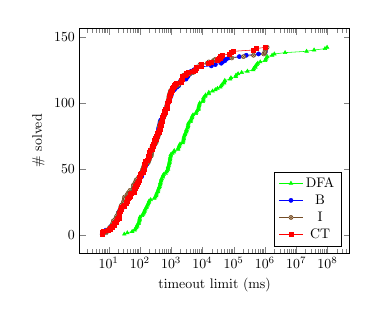
\begin{tikzpicture}[scale=0.5]
      \begin{axis}[
    xmode=log,
    every axis plot/.style={thin},
    xlabel={timeout limit (ms)},
    ylabel={\# solved},
    legend pos=south east
    % table/create on use/cumulative distribution/.style={
    %   create col/expr={\pgfmathaccuma + \thisrow{f(x)}}   
    % }
    ]
    \addplot 
    [mark=triangle*,
    mark size=1.5,
    mark options={solid},
    green] 
    coordinates {
    (31.696, 1)
(39.559, 2)
(56.508, 3)
(68.178, 4)
(70.931, 5)
(75.984, 6)
(81.689, 7)
(82.437, 8)
(90.551, 9)
(92.696, 10)
(96.318, 11)
(97.489, 12)
(98.251, 13)
(100.928, 14)
(116.739, 15)
(124.823, 16)
(132.967, 17)
(139.159, 18)
(141.636, 19)
(149.509, 20)
(161.219, 21)
(165.144, 22)
(176.745, 23)
(182.586, 24)
(193.826, 25)
(196.443, 26)
(220.596, 27)
(287.801, 28)
(307.637, 29)
(331.351, 30)
(335.110, 31)
(344.194, 32)
(377.529, 33)
(378.932, 34)
(389.655, 35)
(410.350, 36)
(423.248, 37)
(438.655, 38)
(450.859, 39)
(454.186, 40)
(475.260, 41)
(483.019, 42)
(493.122, 43)
(544.266, 44)
(544.377, 45)
(568.390, 46)
(658.959, 47)
(704.627, 48)
(733.115, 49)
(790.697, 50)
(796.819, 51)
(799.668, 52)
(839.106, 53)
(863.117, 54)
(884.469, 55)
(886.545, 56)
(921.009, 57)
(927.374, 58)
(928.500, 59)
(970.121, 60)
(970.451, 61)
(1084.311, 62)
(1214.035, 63)
(1256.732, 64)
(1667.050, 65)
(1679.067, 66)
(1790.603, 67)
(1813.082, 68)
(1923.256, 69)
(2334.693, 70)
(2424.581, 71)
(2460.778, 72)
(2524.488, 73)
(2535.289, 74)
(2608.483, 75)
(2727.527, 76)
(2790.777, 77)
(3010.831, 78)
(3089.396, 79)
(3100.186, 80)
(3342.097, 81)
(3421.319, 82)
(3476.286, 83)
(3498.766, 84)
(3603.983, 85)
(4152.208, 86)
(4252.733, 87)
(4414.005, 88)
(4619.485, 89)
(4703.303, 90)
(4995.143, 91)
(6104.482, 92)
(6327.657, 93)
(6680.221, 94)
(7451.205, 95)
(7524.283, 96)
(7577.742, 97)
(7815.366, 98)
(7963.806, 99)
(8190.616, 100)
(10239.338, 101)
(10646.387, 102)
(10743.772, 103)
(10816.354, 104)
(12183.647, 105)
(12608.953, 106)
(15986.466, 107)
(16016.047, 108)
(21085.457, 109)
(25840.612, 110)
(30330.074, 111)
(37303.992, 112)
(39784.632, 113)
(42867.757, 114)
(49654.939, 115)
(49896.816, 116)
(51937.811, 117)
(76626.715, 118)
(81762.693, 119)
(116690.715, 120)
(118979.114, 121)
(138352.575, 122)
(179596.690, 123)
(275896.959, 124)
(422494.853, 125)
(435710.733, 126)
(490650.459, 127)
(500154.998, 128)
(546044.177, 129)
(592457.334, 130)
(707795.890, 131)
(1014847.682, 132)
(1051973.108, 133)
(1109712.990, 134)
(1188811.633, 135)
(1691073.549, 136)
(1998815.209, 137)
(4412151.304, 138)
(21464315.090, 139)
(37446981.305, 140)
(83163795.720, 141)
(97236200.525, 142)
    };

    \addplot 
    [blue,
    mark=*,
    mark size=1.5,
    mark options={solid}]
    coordinates {
    (6.266, 1)
(6.620, 2)
(7.191, 3)
(8.174, 4)
(10.291, 5)
(11.099, 6)
(12.126, 7)
(13.714, 8)
(14.201, 9)
(17.122, 10)
(17.173, 11)
(18.736, 12)
(19.358, 13)
(19.989, 14)
(20.187, 15)
(20.291, 16)
(20.437, 17)
(21.788, 18)
(22.787, 19)
(26.326, 20)
(28.086, 21)
(28.501, 22)
(30.269, 23)
(30.327, 24)
(31.429, 25)
(32.957, 26)
(35.312, 27)
(37.683, 28)
(42.027, 29)
(44.010, 30)
(45.270, 31)
(57.413, 32)
(58.136, 33)
(60.287, 34)
(63.612, 35)
(64.377, 36)
(70.203, 37)
(71.636, 38)
(74.510, 39)
(81.417, 40)
(81.885, 41)
(86.850, 42)
(98.379, 43)
(110.554, 44)
(114.955, 45)
(116.342, 46)
(116.797, 47)
(117.697, 48)
(127.569, 49)
(128.638, 50)
(132.319, 51)
(149.619, 52)
(156.554, 53)
(167.748, 54)
(171.866, 55)
(177.579, 56)
(186.974, 57)
(188.731, 58)
(197.746, 59)
(206.427, 60)
(212.854, 61)
(223.093, 62)
(234.349, 63)
(237.887, 64)
(249.281, 65)
(261.335, 66)
(279.625, 67)
(282.633, 68)
(287.627, 69)
(297.860, 70)
(315.101, 71)
(322.909, 72)
(331.748, 73)
(351.193, 74)
(352.948, 75)
(363.872, 76)
(366.739, 77)
(390.571, 78)
(395.284, 79)
(397.359, 80)
(399.002, 81)
(410.756, 82)
(418.082, 83)
(436.759, 84)
(439.198, 85)
(447.297, 86)
(462.840, 87)
(504.442, 88)
(543.477, 89)
(559.175, 90)
(566.240, 91)
(601.149, 92)
(619.715, 93)
(652.612, 94)
(657.839, 95)
(715.983, 96)
(731.157, 97)
(752.783, 98)
(784.906, 99)
(794.121, 100)
(856.340, 101)
(862.438, 102)
(901.933, 103)
(927.762, 104)
(979.127, 105)
(1000.759, 106)
(1023.428, 107)
(1067.513, 108)
(1074.968, 109)
(1265.279, 110)
(1331.799, 111)
(1538.059, 112)
(1731.374, 113)
(1737.023, 114)
(1790.519, 115)
(1895.419, 116)
(2041.525, 117)
(2975.267, 118)
(3105.441, 119)
(3430.058, 120)
(3574.657, 121)
(3985.434, 122)
(4137.262, 123)
(4364.834, 124)
(5314.336, 125)
(6189.835, 126)
(6463.719, 127)
(19294.688, 128)
(25874.502, 129)
(40075.340, 130)
(44076.314, 131)
(52831.470, 132)
(56117.125, 133)
(69049.283, 134)
(151946.681, 135)
(251788.612, 136)
(624723.233, 137)
(1006224.760, 138)
(1024927.746, 139)
(1025126.900, 140)
(1051096.785, 141)
(1054709.554, 142)
    };

    \addplot [brown!60!black,
    mark options={fill=brown!40},
    mark=otimes*,
    mark size=1.5]
    coordinates {
    (6.225, 1)
(8.252, 2)
(8.866, 3)
(8.903, 4)
(10.276, 5)
(10.793, 6)
(12.246, 7)
(12.967, 8)
(13.482, 9)
(13.873, 10)
(14.125, 11)
(15.975, 12)
(17.388, 13)
(17.590, 14)
(18.641, 15)
(20.043, 16)
(20.476, 17)
(21.613, 18)
(23.615, 19)
(24.164, 20)
(24.372, 21)
(24.882, 22)
(26.053, 23)
(29.400, 24)
(29.513, 25)
(30.549, 26)
(31.898, 27)
(32.205, 28)
(32.366, 29)
(39.353, 30)
(39.524, 31)
(42.127, 32)
(45.853, 33)
(48.185, 34)
(60.297, 35)
(60.940, 36)
(61.286, 37)
(61.970, 38)
(67.684, 39)
(71.354, 40)
(74.374, 41)
(76.755, 42)
(86.492, 43)
(92.532, 44)
(102.074, 45)
(107.118, 46)
(110.458, 47)
(119.452, 48)
(120.692, 49)
(122.537, 50)
(130.211, 51)
(131.757, 52)
(139.069, 53)
(139.341, 54)
(184.184, 55)
(187.471, 56)
(198.576, 57)
(201.040, 58)
(207.945, 59)
(229.958, 60)
(232.188, 61)
(233.976, 62)
(239.163, 63)
(240.688, 64)
(241.932, 65)
(243.311, 66)
(245.547, 67)
(265.954, 68)
(292.029, 69)
(328.546, 70)
(334.072, 71)
(336.358, 72)
(350.752, 73)
(375.324, 74)
(379.234, 75)
(396.967, 76)
(401.683, 77)
(401.895, 78)
(405.570, 79)
(411.227, 80)
(417.570, 81)
(419.966, 82)
(421.977, 83)
(456.664, 84)
(458.121, 85)
(467.458, 86)
(514.809, 87)
(537.183, 88)
(573.529, 89)
(585.083, 90)
(628.983, 91)
(629.151, 92)
(638.579, 93)
(655.494, 94)
(683.596, 95)
(719.854, 96)
(720.103, 97)
(726.177, 98)
(743.018, 99)
(776.859, 100)
(788.068, 101)
(801.667, 102)
(840.869, 103)
(844.819, 104)
(845.660, 105)
(882.665, 106)
(896.694, 107)
(936.968, 108)
(941.257, 109)
(1025.243, 110)
(1127.272, 111)
(1290.616, 112)
(1527.467, 113)
(1798.817, 114)
(1803.072, 115)
(1966.245, 116)
(2089.371, 117)
(2225.216, 118)
(2378.815, 119)
(2497.087, 120)
(2503.823, 121)
(3943.794, 122)
(5004.718, 123)
(5143.946, 124)
(5663.752, 125)
(6369.410, 126)
(6913.053, 127)
(8260.886, 128)
(8382.946, 129)
(14367.240, 130)
(16013.595, 131)
(22433.224, 132)
(26100.534, 133)
(86936.175, 134)
(206857.036, 135)
(432302.057, 136)
(923791.300, 137)
(1001275.049, 138)
(1005552.392, 139)
(1024252.398, 140)
(1082346.127, 141)
(1174868.682, 142)
    };

    \addplot 
    [red,
    mark size=1.5,
    mark=square*]
    coordinates {
    (6.328, 1)
(6.344, 2)
(6.785, 3)
(9.703, 4)
(11.389, 5)
(12.785, 6)
(13.199, 7)
(14.710, 8)
(15.330, 9)
(17.053, 10)
(17.466, 11)
(18.730, 12)
(21.191, 13)
(21.458, 14)
(22.190, 15)
(22.321, 16)
(22.429, 17)
(23.230, 18)
(23.566, 19)
(24.810, 20)
(24.843, 21)
(30.529, 22)
(31.162, 23)
(35.615, 24)
(37.410, 25)
(38.475, 26)
(38.831, 27)
(43.209, 28)
(45.793, 29)
(47.775, 30)
(48.066, 31)
(53.755, 32)
(65.633, 33)
(66.267, 34)
(66.798, 35)
(69.198, 36)
(73.621, 37)
(77.636, 38)
(83.309, 39)
(87.127, 40)
(87.800, 41)
(92.901, 42)
(93.082, 43)
(98.471, 44)
(101.548, 45)
(102.853, 46)
(112.950, 47)
(126.755, 48)
(126.916, 49)
(133.777, 50)
(136.483, 51)
(139.301, 52)
(141.708, 53)
(142.901, 54)
(147.720, 55)
(151.267, 56)
(167.047, 57)
(180.053, 58)
(185.002, 59)
(192.458, 60)
(199.346, 61)
(200.444, 62)
(205.194, 63)
(211.032, 64)
(245.046, 65)
(247.635, 66)
(258.985, 67)
(273.140, 68)
(274.226, 69)
(289.992, 70)
(293.258, 71)
(296.666, 72)
(320.259, 73)
(325.794, 74)
(331.950, 75)
(359.459, 76)
(369.740, 77)
(401.942, 78)
(428.598, 79)
(439.186, 80)
(443.919, 81)
(451.155, 82)
(465.721, 83)
(486.636, 84)
(496.533, 85)
(507.498, 86)
(509.344, 87)
(518.391, 88)
(534.298, 89)
(549.969, 90)
(554.731, 91)
(594.595, 92)
(623.445, 93)
(624.194, 94)
(658.888, 95)
(748.721, 96)
(754.742, 97)
(754.776, 98)
(757.089, 99)
(766.244, 100)
(789.618, 101)
(856.352, 102)
(878.697, 103)
(882.688, 104)
(885.633, 105)
(948.909, 106)
(961.811, 107)
(1025.381, 108)
(1027.979, 109)
(1068.881, 110)
(1096.069, 111)
(1141.179, 112)
(1263.836, 113)
(1363.480, 114)
(1444.963, 115)
(2086.545, 116)
(2104.289, 117)
(2266.072, 118)
(2315.715, 119)
(2337.155, 120)
(2809.498, 121)
(3062.328, 122)
(3613.655, 123)
(4962.131, 124)
(5757.448, 125)
(6278.281, 126)
(6458.606, 127)
(9074.926, 128)
(9388.538, 129)
(15237.846, 130)
(19012.640, 131)
(29844.102, 132)
(32057.652, 133)
(36009.393, 134)
(38516.958, 135)
(44360.448, 136)
(70712.723, 137)
(84815.013, 138)
(99208.278, 139)
(426595.818, 140)
(513749.533, 141)
(1012388.065, 142)
    };
    \legend{DFA,B,I,CT}
  \end{axis}

    \end{tikzpicture}
    &
      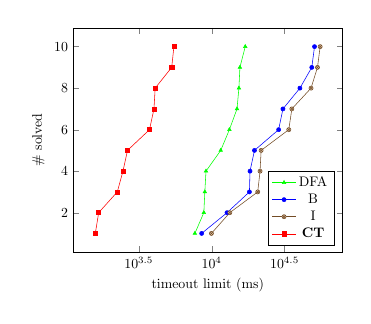
\begin{tikzpicture}[scale=0.5]
        \begin{axis}[
    xmode=log,
    every axis plot/.style={thin},
    xlabel={timeout limit (ms)},
    ylabel={\# solved},
    legend pos=south east
    % table/create on use/cumulative distribution/.style={
    %   create col/expr={\pgfmathaccuma + \thisrow{f(x)}}   
    % }
    ]
    \addplot 
    [mark=triangle*,
    mark size=1.5,
    mark options={solid},
    green] 
    coordinates {
    (7669.883, 1)
(8836.338, 2)
(8977.330, 3)
(9140.777, 4)
(11537.562, 5)
(13231.384, 6)
(14923.762, 7)
(15381.136, 8)
(15623.402, 9)
(16994.255, 10)
    };

    \addplot 
    [blue,
    mark=*,
    mark size=1.5,
    mark options={solid}]
    coordinates {
    (8538.228, 1)
(12749.685, 2)
(18156.956, 3)
(18327.323, 4)
(19669.292, 5)
(28802.590, 6)
(30835.715, 7)
(40301.654, 8)
(48620.995, 9)
(50774.009, 10)
    };

    \addplot [brown!60!black,
    mark options={fill=brown!40},
    mark=otimes*,
    mark size=1.5]
    coordinates {
    (9960.047, 1)
(13326.927, 2)
(20700.530, 3)
(21474.840, 4)
(21842.271, 5)
(33817.893, 6)
(35489.987, 7)
(48049.593, 8)
(53196.297, 9)
(55499.785, 10)
    };

    \addplot 
    [red,
    mark size=1.5,
    mark=square*]
    coordinates {
    (1591.239, 1)
(1678.457, 2)
(2251.773, 3)
(2462.919, 4)
(2646.514, 5)
(3745.993, 6)
(4020.526, 7)
(4095.836, 8)
(5320.617, 9)
(5507.353, 10)
    };
    \legend{DFA,B,I,\textbf{CT}}
  \end{axis}

      \end{tikzpicture} \\
  \end{tabular}
\end{frame}

\begin{frame}
  \frametitle{Results}
  \begin{itemize}
    \item On all series, CT either outperforms or performs as well as the existing
      propagators for~\Table
    \item DFA overall slowest, but fastest on some series
    \item CT has largest performance gains on series with large tables
  \end{itemize}
\end{frame}

\section{Summary and Conclusions}

\begin{frame}
  \frametitle{Summary and Conclusions}
  \begin{itemize}
  \item   What I have done:
    \begin{itemize}
    \item Implemented Compact-Table (CT) in Gecode
    \item Compared CT against existing propagators for \Table,
      and with \Constraint{Regular}
    \end{itemize}
  \item   The results:
    \begin{itemize}
      \item CT seems to outperform existing propagators for \Table
    \end{itemize}
    % \item Remains to be done:
    %   \begin{itemize}
    %     \item Find a bug
    %   \end{itemize}
    \item Future work:
      \begin{itemize}
      \item This project is to be seen as a proof of concept - not a final version
      \item Inclusion into Gecode?
      \item Implement and evaluate generalisations of CT described
        in~\cite{DBLP:conf/aaai/VerhaegheLS17}
      \end{itemize}
  
  \end{itemize}
\end{frame}

\begin{frame}
  \frametitle{References}
  \printbibliography
  %\begin{thebibliography}{9}
    
  %\bibitem[Demeulenaere, Hartert, Lecoutre, Perez, Perron, R{\'{e}}gin, and Schaus @ CP 2016]{CTpaper} Demeulenaere, J. and Hartert, R. and Lecoutre, C. and Perez, G. and Perron, L. and R{\'{e}}gin, J.C. and Schaus, P.
%   \bibitem[1]{CTpaper} Demeulenaere, J. and Hartert, R. and Lecoutre, C. and Perez, G. and Perron, L. and R{\'{e}}gin, J.C. and Schaus, P.
%     \newblock Compact-Table: Efficiently Filtering Table Constraints with Reversible
%     Sparse Bit-Sets
%     \newblock \emph{Proceedings of CP 2016}, Lecture Notes in Computer Science 9892, pages 207--223. Springer, 2016.
    

% %  \bibitem[Verhaeghe, Lecoutre, and Schaus @ AAAI 2017]{CTpaper2} Verhaeghe, H{\'{e}}l{\`{e}}ne and Lecoutre, Christophe and Schaus, Pierre
%   \bibitem[2]{CTpaper2} Verhaeghe, H{\'{e}}l{\`{e}}ne and Lecoutre, Christophe and Schaus, Pierre
%     \newblock Extending Compact-Table to Negative and Short Tables,
%     \emph{Proceedings of AAAI 2017}, AAAI 2017, pages 3951--3957. AAAI Press, 2017.
               
  %\end{thebibliography}

\end{frame}

\end{document}
